\documentclass[12pt,letterpaper]{article}
\usepackage[utf8]{inputenc}
\usepackage[spanish]{babel}
\usepackage{graphicx}
\usepackage[hidelinks]{hyperref}
\usepackage{hyperref}
\usepackage[left=2cm,right=2cm,top=2.5cm,bottom=2cm]{geometry}
\usepackage{graphicx} % figuras
\usepackage{float} % para usar [H]
\usepackage{amsmath}
\usepackage{stackrel} 
\usepackage{multicol}
\usepackage{multirow}
\usepackage{fancyhdr}
\usepackage[usenames,dvipsnames,svgnames,table]{xcolor}
\usepackage[document]{ragged2e}
\usepackage{enumerate} % enumerados
\renewcommand{\labelitemi}{$-$}
\renewcommand{\labelitemii}{$\cdot$}
\newcommand\tab[1][1cm]{\hspace*{#1}}

\definecolor{amarillo}{RGB}{255,255,0}
\definecolor{rojo}{RGB}{255,0,0}
\definecolor{azul}{RGB}{0,0,255}
\definecolor{verdeClaro}{RGB}{0,255,0}

%encabezado
\pagestyle{fancy}
\lhead{\begin{picture}(0,0) \put(0,0){
\includegraphics[width=10mm]{./img/logo}} \end{picture}}
\chead{\hspace{1cm}\vspace{0.2cm}INFORME DE LABORATORIO N° 02 - VISUALIZACION DE DATOS CON QLIK SENSE}
\rhead{}

\begin{document}
    \begin{titlepage}
        \begin{center}
            \begin{figure}[htb]
                \begin{center}
                    
\includegraphics[width=3.5cm]{./img/logo}
                \end{center}
            \end{figure}
            \vspace*{0.15in}
            \begin{Large}
                \textbf{UNIVERSIDAD PRIVADA DE TACNA}\\
            \end{Large}
            \vspace*{0.15in}
            \begin{Large}
                \textbf{FACULTAD DE INGENIERIA} \\
            \end{Large}
            \vspace*{0.1in}
            \begin{Large}
                \textbf{Escuela Profesional de Ingeniería de Sistemas} \\
            \end{Large}
            \vspace*{0.3in}
            \begin{Large}
                \textbf{INFORME DE LABORATORIO N°02}\\
                \textbf{“VISUALIZACION DE DATOS CON QLIK SENSE}\\
            \end{Large}
            \vspace*{0.2in}
            \begin{Large}
                \textbf{CURSO:} \\
            \end{Large}
            \vspace*{0.1in}
            \begin{large}
                Inteligencia de Negocios\\
            \end{large}
            \vspace*{0.2in}
            \begin{Large}
                \textbf{DOCENTE:} \\
            \end{Large}
            \vspace*{0.1in}
            \begin{large}
                Mag. Patrick Jose Cuadros Quiroga\\
            \end{large}
            \vspace*{0.3in}
            \begin{large}
                \textbf{ALUMNO:} \\
                \begin{flushleft}
                    Gutierrez Ponce, José Carlos  		\hfill	(2017059277) \\
                \end{flushleft}
            \end{large}
            \vspace*{1.3in}
            \begin{large}
                Tacna - Perú\\
            \end{large}
            \vspace*{0.1in}
            \begin{large}
                2021\\
            \end{large}
        \end{center}
    \end{titlepage}
    \include{Secciones/articulo}
    %%%%%%%%%%%%%%%%%%%%%%%%%%%%%%%%%%%%%%%%%%%%%%%%%%%%%%%%%%%%%%%%%%%%%%%%%%%%%%%%%%%%%%%%%%%%%%%%%%%%%%%%%%%%%%%%%%%%%%%%%%%%%%%%%%%%%%%%%%%%%%%%%%%%%%%%%%%%%%%%%%%%%%%%%%%%%%%%%%%%%%%%%%%%%%%%%%%%%%%%%%%%%%%%%%%%%%%%%%%%%%%%%%%%%%%%%%%%%%%%%%%%%%%%%%%%%%%%%%%%%%%%%%%%%%%%%%%%%%%%%%%%%%%%%%%%%%%%%%%%%%%%%%%%%%%%%%%%%%%%%%%%%%%%%%%%%%%%%%%%%%%%%%%%%%%%%%%%%%%%%%%%%%%%%%%%%%%%%%%%%%%%%%%%%%%%%%%%%%%%%%%%%%%%%%%%%%%%%%%%%%%%%%%%%%%%%%%%%%%%%%%%%%%%%%%%%%%%%%%%%%%%%%%%%%%%%%%%%%%%%%%%%%%%%%%%%%%
    \newpage
    \tableofcontents
    \justify
    %%%%%%%%%%%%%%%%%%%%%%%%%%%%%%%%%%%%%%%%%%%%%%%%%%%%%%%%%%%%%%%%%%%%%%%%%%%%%%%%%%%%%%%%%%%%%%%%%%%%%%%%%%%%%%%%%%%%%%%%%%%%%%%%%%%%%%%%%%%%%%%%%%%%%%%%%%%%%%%%%%%%%%%%%%%%%%%%%%%%%%%%%%%%%%%%%%%%%%%%%%%%%%%%%%%%%%%%%%%%%%%%%%%%%%%%%%%%%%%%%%%%%%%%%%%%%%%%%%%%%%%%%%%%%%%%%%%%%%%%%%%%%%%%%%%%%%%%%%%%%%%%%%%%%%%%%%%%%%%%%%%%%%%%%%%%%%%%%%%%%%%%%%%%%%%%%%%%%%%%%%%%%%%%%%%%%%%%%%%%%%%%%%%%%%%%%%%%%%%%%%%%%%%%%%%%%%%%%%%%%%%%%%%%%%%%%%%%%%%%%%%%%%%%%%%%%%%%%%%%%%%%%%%%%%%%%%%%%%%%%%%%%%%%%%%%%%%
    \newpage
    \begin{LARGE}
        \begin{center}
            \textbf{VISUALIZACION DE DATOS CON QLIK SENSE} \\
        \end{center}
    \end{LARGE}
    %%%%%%%%%%%%%%%%%%%%%%%%%%%%%%%%%%%%%%%%%%%%%%%%%%%%%%%%%%%%%%%%%%%%%%%%%%%%%%%%%%%%%%%%%%%%%%%%%%%%%%%%%%%%%%%%%%%%%%%%%%%%%%%%%%%%%%%%%%%%%%%%%%%%%%%%%%%%%%%%%%%%%%%%%%%%%%%%%%%%%%%%%%%%%%%%%%%%%%%%%%%%%%%%%%%%%%%%%%%%%%%%%%%%%%%%%%%%%%%%%%%%%%%%%%%%%%%%%%%%%%%%%%%%%%%%%%%%%%%%%%%%%%%%%%%%%%%%%%%%%%%%%%%%%%%%%%%%%%%%%%%%%%%%%%%%%%%%%%%%%%%%%%%%%%%%%%%%%%%%%%%%%%%%%%%%%%%%%%%%%%%%%%%%%%%%%%%%%%%%%%%%%%%%%%%%%%%%%%%%%%%%%%%%%%%%%%%%%%%%%%%%%%%%%%%%%%%%%%%%%%%%%%%%%%%%%%%%%%%%%%%%%%%%%%%%%%%
    \section{OBJETIVOS}
    \begin{itemize}
        \item Crear una aplicación diseñada para evaluar las ventas en diferentes países, considerar las tendencias de ventas a lo largo del tiempo y descubrir y centrarse en las categorías de productos con bajos totales de ventas.
    \end{itemize}
    %%%%%%%%%%%%%%%%%%%%%%%%%%%%%%%%%%%%%%%%%%%%%%%%%%%%%%%%%%%%%%%%%%%%%%%%%%%%%%%%%%%%%%%%%%%%%%%%%%%%%%%%%%%%%%%%%%%%%%%%%%%%%%%%%%%%%%%%%%%%%%%%%%%%%%%%%%%%%%%%%%%%%%%%%%%%%%%%%%%%%%%%%%%%%%%%%%%%%%%%%%%%%%%%%%%%%%%%%%%%%%%%%%%%%%%%%%%%%%%%%%%%%%%%%%%%%%%%%%%%%%%%%%%%%%%%%%%%%%%%%%%%%%%%%%%%%%%%%%%%%%%%%%%%%%%%%%%%%%%%%%%%%%%%%%%%%%%%%%%%%%%%%%%%%%%%%%%%%%%%%%%%%%%%%%%%%%%%%%%%%%%%%%%%%%%%%%%%%%%%%%%%%%%%%%%%%%%%%%%%%%%%%%%%%%%%%%%%%%%%%%%%%%%%%%%%%%%%%%%%%%%%%%%%%%%%%%%%%%%%%%%%%%%%%%%%%%%
    \section{REQUERIMIENTOS}
    \begin{itemize}
        \item Conocimientos\\
        Para el desarrollo de esta práctica se requerirá de los siguientes conocimientos básicos:
        \begin{itemize} 
            \item Conocimientos básicos en el uso de Qlik Sense.
        \end{itemize}
        \item Hardware
        \begin{itemize}
            \item CPU SLAT-capable feature.
            \item Al menos 4GB de RAM.
        \end{itemize}
        \item Software\\
        Así mismo se necesitan los siguientes aplicativos
        \begin{itemize}
            \item Windows 10 64bit: Pro, Enterprise o Education (1607 Anniversary Update, Build 14393 o Superior) 
            \item Navegador de Internet (\textcolor{azul}{\url{https://www.google.com/intl/es-419/chrome/}}).
        \end{itemize}
    \end{itemize}
    %%%%%%%%%%%%%%%%%%%%%%%%%%%%%%%%%%%%%%%%%%%%%%%%%%%%%%%%%%%%%%%%%%%%%%%%%%%%%%%%%%%%%%%%%%%%%%%%%%%%%%%%%%%%%%%%%%%%%%%%%%%%%%%%%%%%%%%%%%%%%%%%%%%%%%%%%%%%%%%%%%%%%%%%%%%%%%%%%%%%%%%%%%%%%%%%%%%%%%%%%%%%%%%%%%%%%%%%%%%%%%%%%%%%%%%%%%%%%%%%%%%%%%%%%%%%%%%%%%%%%%%%%%%%%%%%%%%%%%%%%%%%%%%%%%%%%%%%%%%%%%%%%%%%%%%%%%%%%%%%%%%%%%%%%%%%%%%%%%%%%%%%%%%%%%%%%%%%%%%%%%%%%%%%%%%%%%%%%%%%%%%%%%%%%%%%%%%%%%%%%%%%%%%%%%%%%%%%%%%%%%%%%%%%%%%%%%%%%%%%%%%%%%%%%%%%%%%%%%%%%%%%%%%%%%%%%%%%%%%%%%%%%%%%%%%%%%%
    \section{CONSIDERACIONES INICIALES}
    \begin{itemize}
        \item Tener una cuenta en Qlik.
        \item Tener el archivo ExerciseDara.xlsx, se puede descargar desde \textcolor{azul}{\href{https://learning.qlik.com/mod/resource/view.php?id=22519}{aca}}
    \end{itemize}
    %%%%%%%%%%%%%%%%%%%%%%%%%%%%%%%%%%%%%%%%%%%%%%%%%%%%%%%%%%%%%%%%%%%%%%%%%%%%%%%%%%%%%%%%%%%%%%%%%%%%%%%%%%%%%%%%%%%%%%%%%%%%%%%%%%%%%%%%%%%%%%%%%%%%%%%%%%%%%%%%%%%%%%%%%%%%%%%%%%%%%%%%%%%%%%%%%%%%%%%%%%%%%%%%%%%%%%%%%%%%%%%%%%%%%%%%%%%%%%%%%%%%%%%%%%%%%%%%%%%%%%%%%%%%%%%%%%%%%%%%%%%%%%%%%%%%%%%%%%%%%%%%%%%%%%%%%%%%%%%%%%%%%%%%%%%%%%%%%%%%%%%%%%%%%%%%%%%%%%%%%%%%%%%%%%%%%%%%%%%%%%%%%%%%%%%%%%%%%%%%%%%%%%%%%%%%%%%%%%%%%%%%%%%%%%%%%%%%%%%%%%%%%%%%%%%%%%%%%%%%%%%%%%%%%%%%%%%%%%%%%%%%%%%%%%%%%%%
    \newpage
    \section{DESARROLLO}
    %%%%%%%%%%%%%%%%%%%%%%%%%%%%%%%%%%%%%%%%%%%%%%%%%%%%%%%%%%%%%%%%%%%%%%%%%%%%%%%%%%%%%%%%%%%%%%%%%%%%%%%%%%%%%%%%%%%%%%%%%%%%%%%%%%%%%%%%%%%%%%%%%%%%%%%%%%%%%%%%%%%%%%%%%%%%%%%%%%%%%%%%%%%%%%%%%%%%%%%%%%%%%%%%%%%%%%%%%%%%%%%%%%%%%%%%%%%%%%%%%%%%%%%%%%%%%%%%%%%%%%%%%%%%%%%%%%%%%%%%%%%%%%%%%%%%%%%%%%%%%%%%%%%%%%%%%%%%%%%%%%%%%%%%%%%%%%%%%%%%%%%%%%%%%%%%%%%%%%%%%%%%%%%%%%%%%%%%%%%%%%%%%%%%%%%%%%%%%%%%%%%%%%%%%%%%%%%%%%%%%%%%%%%%%%%%%%%%%%%%%%%%%%%%%%%%%%%%%%%%%%%%%%%%%%%%%%%%%%%%%%%%%%%%%%%%%%%
    \subsection{Crea una nueva aplicación}
    \begin{enumerate}[\tab 1.]
        \item Ingresar a \textcolor{azul}{\url{https://nwwo7wskldu3fck.us.qlikcloud.com/}}.
        \begin{center}
            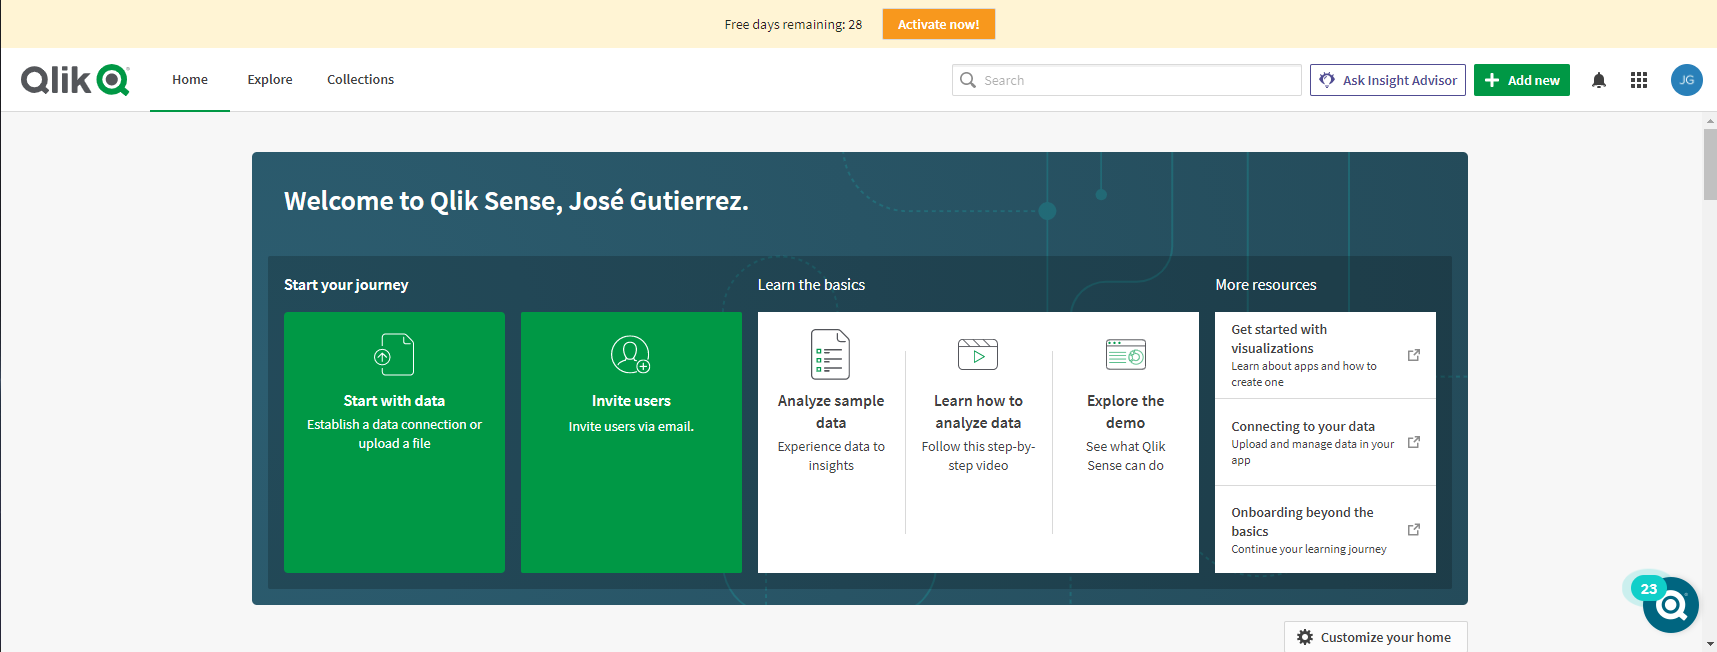
\includegraphics[width=13cm]{./img/img1.png}
        \end{center}
        \item Crear una nueva app.
        \begin{center}
            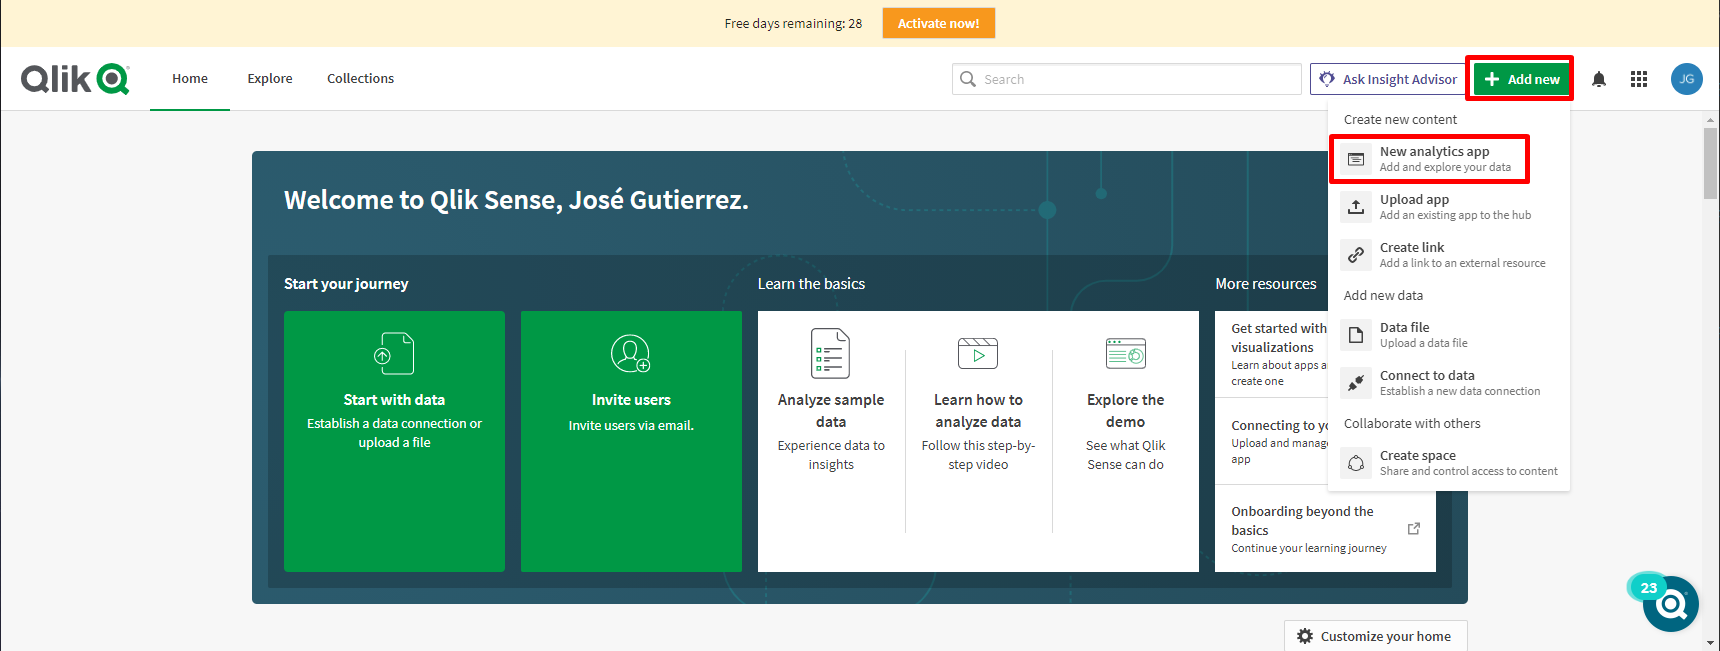
\includegraphics[width=13cm]{./img/img2.png}
        \end{center}
        \begin{itemize}
            \item Colocar el nombre \textit{\textbf{"My Sales Analysis"}} y hacer clic en el boton \textbf{Create}.
            \begin{center}
                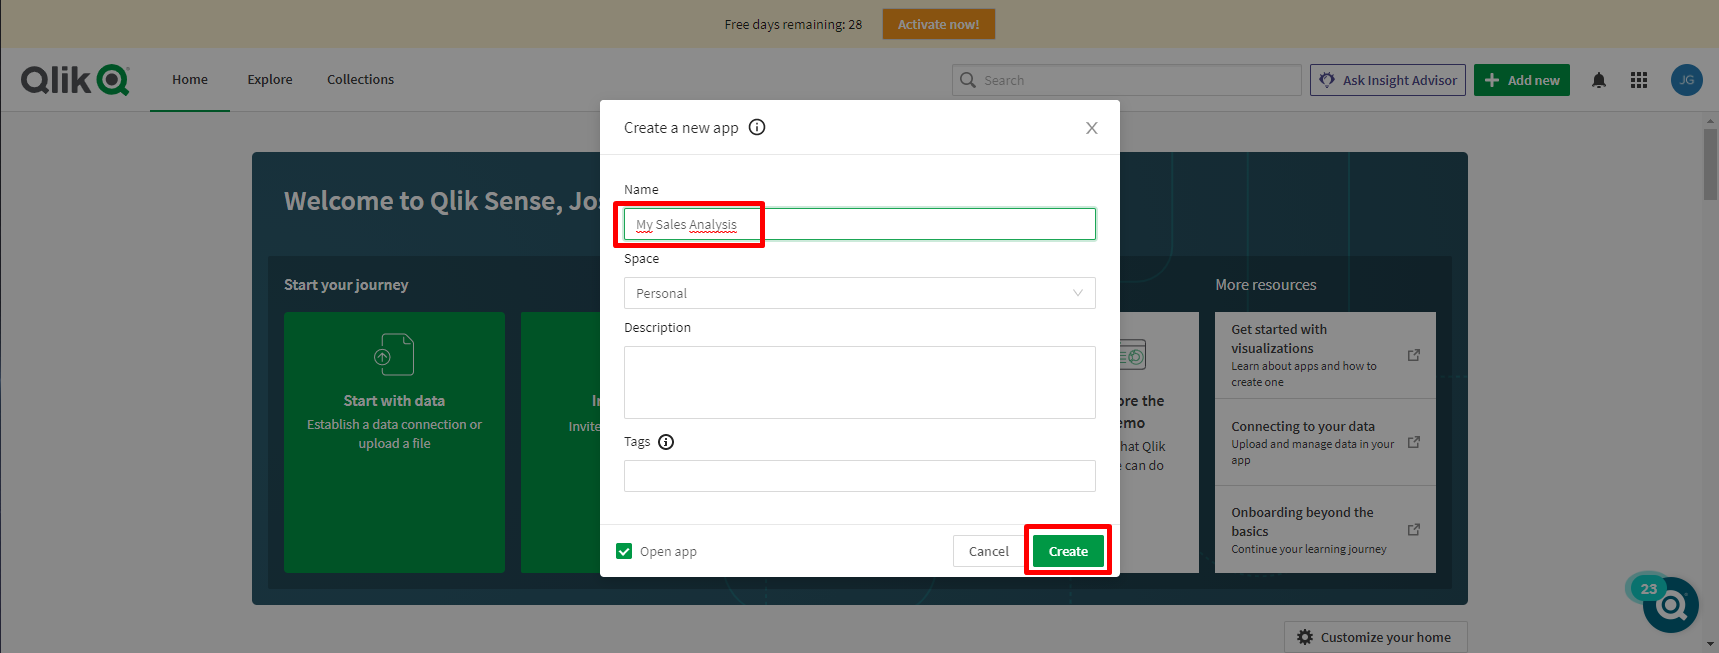
\includegraphics[width=13cm]{./img/img2.1.png}
            \end{center}
            \item Abrir la app creada.
            \begin{center}
                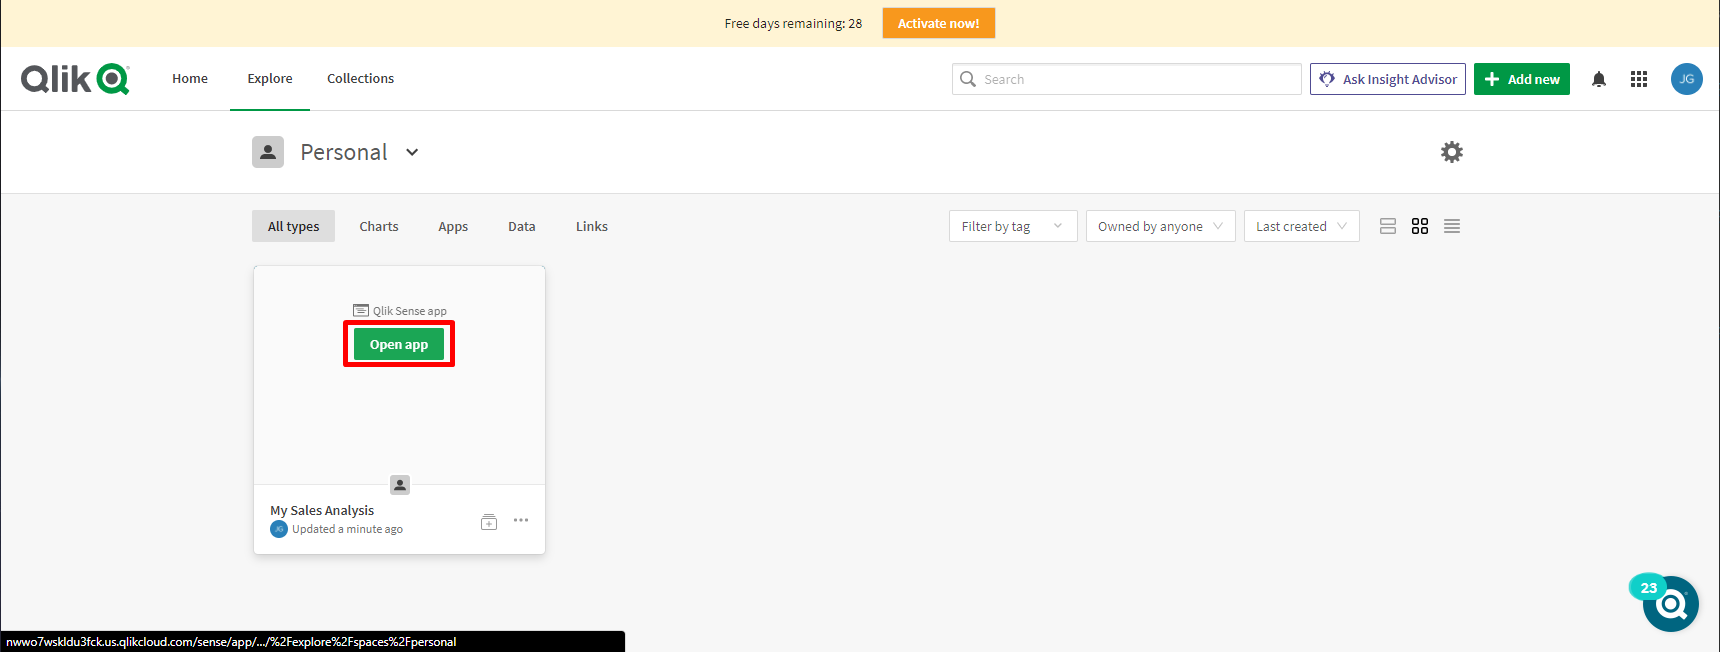
\includegraphics[width=13cm]{./img/img2.2.png}
            \end{center}
        \end{itemize}
    \end{enumerate}
    %%%%%%%%%%%%%%%%%%%%%%%%%%%%%%%%%%%%%%%%%%%%%%%%%%%%%%%%%%%%%%%%%%%%%%%%%%%%%%%%%%%%%%%%%%%%%%%%%%%%%%%%%%%%%%%%%%%%%%%%%%%%%%%%%%%%%%%%%%%%%%%%%%%%%%%%%%%%%%%%%%%%%%%%%%%%%%%%%%%%%%%%%%%%%%%%%%%%%%%%%%%%%%%%%%%%%%%%%%%%%%%%%%%%%%%%%%%%%%%%%%%%%%%%%%%%%%%%%%%%%%%%%%%%%%%%%%%%%%%%%%%%%%%%%%%%%%%%%%%%%%%%%%%%%%%%%%%%%%%%%%%%%%%%%%%%%%%%%%%%%%%%%%%%%%%%%%%%%%%%%%%%%%%%%%%%%%%%%%%%%%%%%%%%%%%%%%%%%%%%%%%%%%%%%%%%%%%%%%%%%%%%%%%%%%%%%%%%%%%%%%%%%%%%%%%%%%%%%%%%%%%%%%%%%%%%%%%%%%%%%%%%%%%%%%%%%%%
    \subsection{Cargar datos}
    \begin{enumerate}[\tab 1.]
        \item Utilice el mosaico \textbf{Agregar datos de archivos y otras fuentes} para agregar los datos del Excel a la aplicación (\textit{desde el archivo ExerciseData.xlsx}).
        \begin{center}
            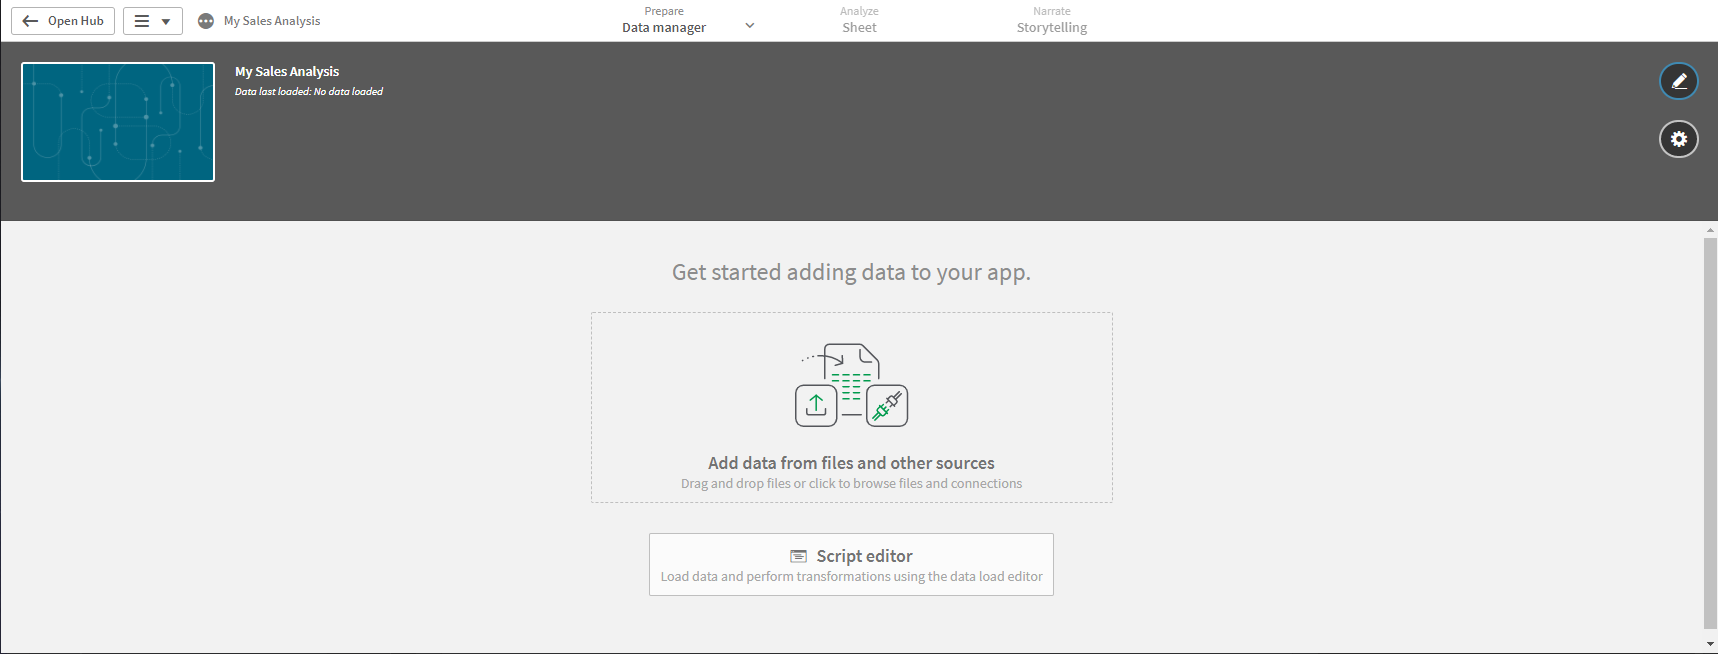
\includegraphics[width=13cm]{./img/img3.png}
        \end{center}
        \begin{itemize}
            \item Cargue todos los campos de la hoja de cálculo, haciendo clic en el botón \textbf{Next}.
            \begin{center}
                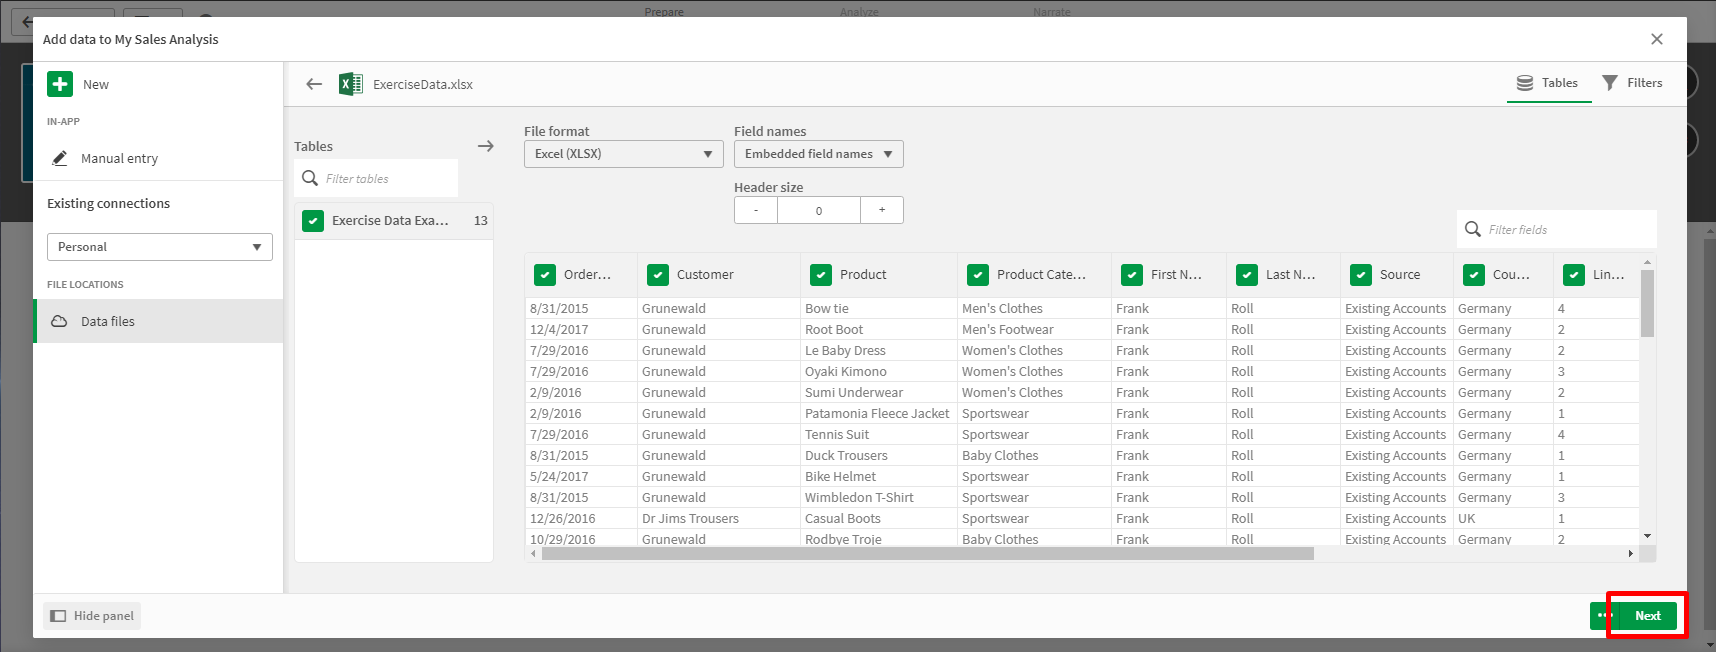
\includegraphics[width=13cm]{./img/img3.1.png}
            \end{center}
        \end{itemize}
    \end{enumerate}
    %%%%%%%%%%%%%%%%%%%%%%%%%%%%%%%%%%%%%%%%%%%%%%%%%%%%%%%%%%%%%%%%%%%%%%%%%%%%%%%%%%%%%%%%%%%%%%%%%%%%%%%%%%%%%%%%%%%%%%%%%%%%%%%%%%%%%%%%%%%%%%%%%%%%%%%%%%%%%%%%%%%%%%%%%%%%%%%%%%%%%%%%%%%%%%%%%%%%%%%%%%%%%%%%%%%%%%%%%%%%%%%%%%%%%%%%%%%%%%%%%%%%%%%%%%%%%%%%%%%%%%%%%%%%%%%%%%%%%%%%%%%%%%%%%%%%%%%%%%%%%%%%%%%%%%%%%%%%%%%%%%%%%%%%%%%%%%%%%%%%%%%%%%%%%%%%%%%%%%%%%%%%%%%%%%%%%%%%%%%%%%%%%%%%%%%%%%%%%%%%%%%%%%%%%%%%%%%%%%%%%%%%%%%%%%%%%%%%%%%%%%%%%%%%%%%%%%%%%%%%%%%%%%%%%%%%%%%%%%%%%%%%%%%%%%%%%%%
    \subsection{Revisar datos}
    \begin{enumerate}[\tab 1.]
        \item Utilice el menú de acceso rápido para navegar a la vista del Administrador de datos y obtener más información sobre esta tabla.
        \begin{center}
            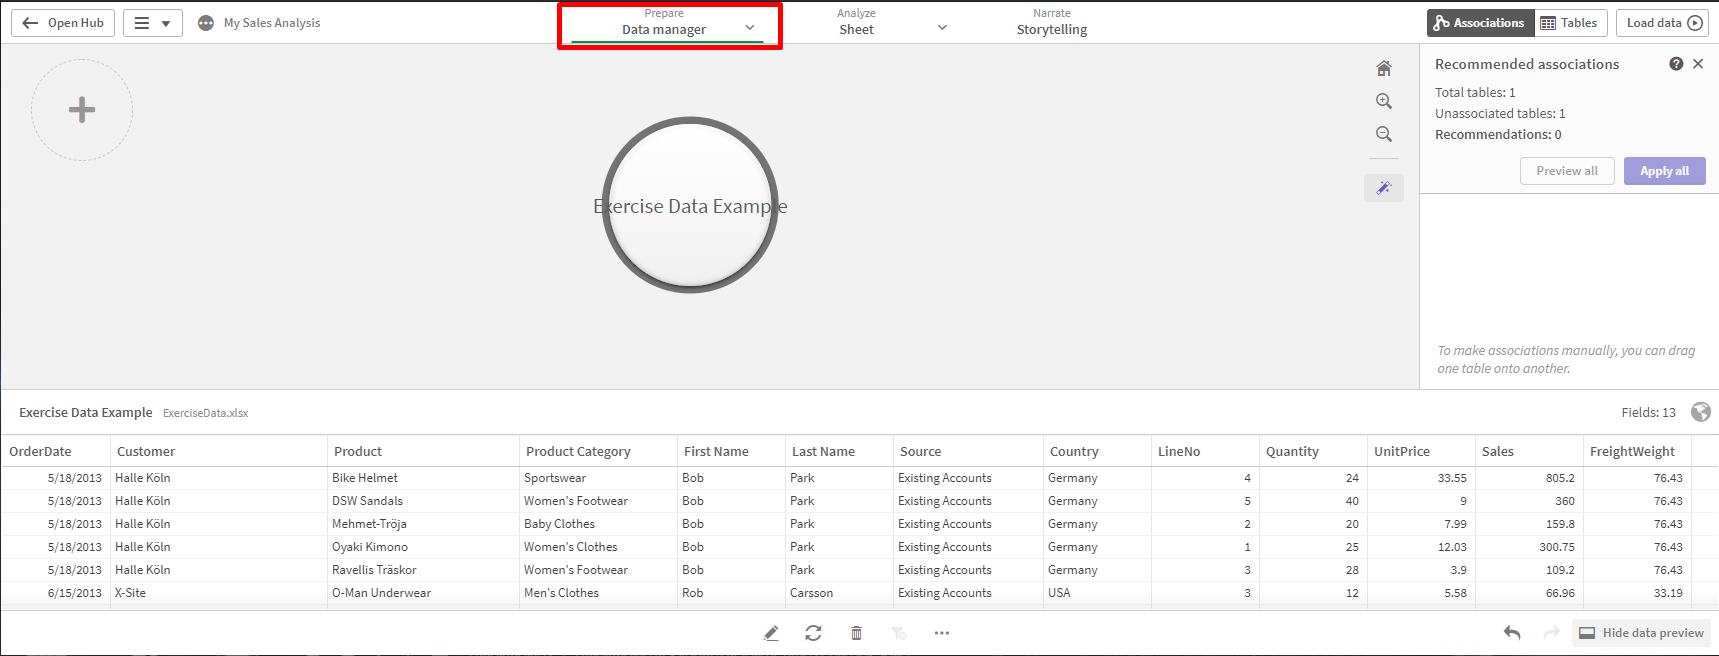
\includegraphics[width=13cm]{./img/img4.png}
        \end{center}
        \item Abra la vista del editor de tablas del administrador de datos haciendo clic en el ícono de \textbf{lapiz} en la parte inferior de la vista.
        \begin{center}
            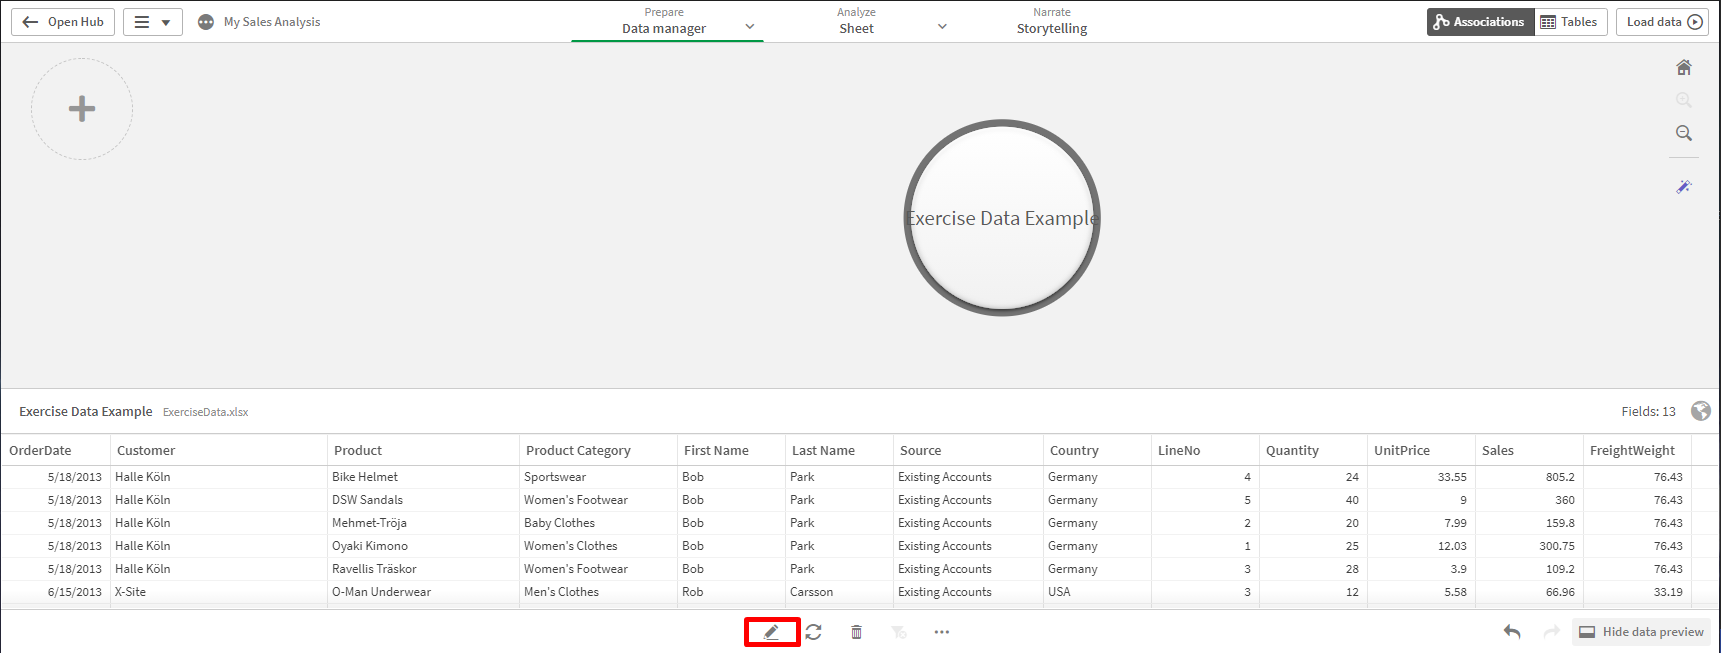
\includegraphics[width=13cm]{./img/img5.png}
        \end{center}
        \item Haga clic en los campos indicados y vea la tarjeta de resumen para responder las siguientes preguntas:
        \begin{itemize}
            \item ¿Cuántos valores de \textit{\textbf{Country}} distintos están presentes en esta tabla?
            \begin{center}
                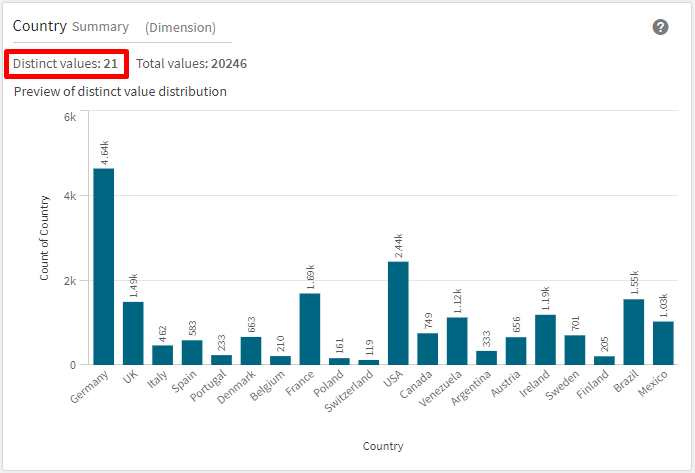
\includegraphics[width=13cm]{./img/img6.1.png}
            \end{center}
            \item ¿Cuántos valores distintos hay para la \textit{\textbf{Product Category}}?
            \begin{center}
                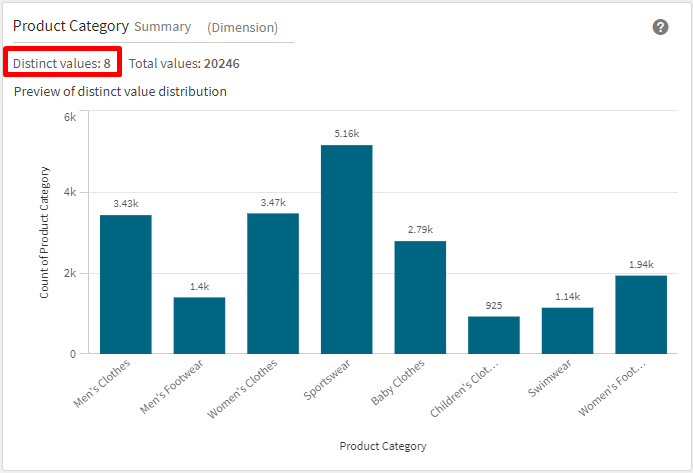
\includegraphics[width=13cm]{./img/img6.2.png}
            \end{center}
            \item ¿Cuántos valores distintos hay para el campo \textit{\textbf{Product}}?
            \begin{center}
                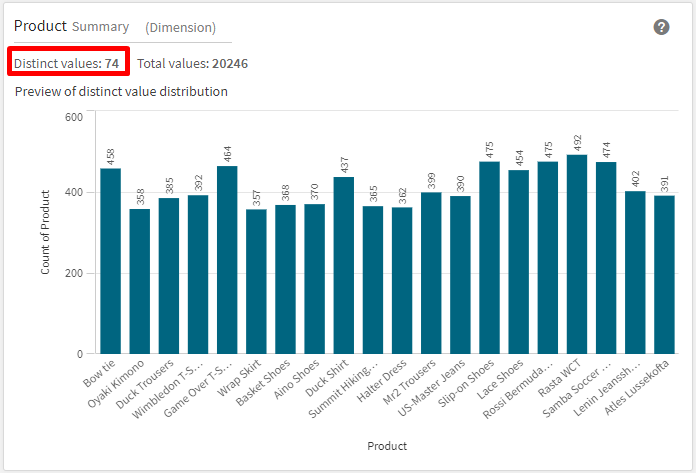
\includegraphics[width=13cm]{./img/img6.3.png}
            \end{center}
            \item ¿Cuántos valores distintos hay para el campo \textit{\textbf{Source}}?
            \begin{center}
                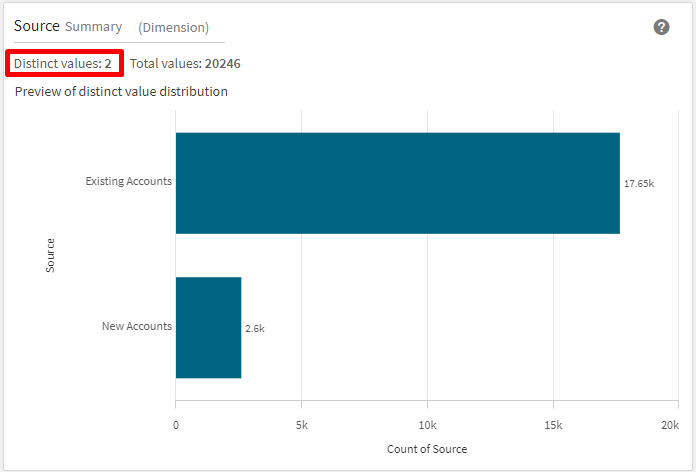
\includegraphics[width=13cm]{./img/img6.4.png}
            \end{center}
            \item ¿Cuáles son esos dos valores del campo \textit{\textbf{Source}}?
            \begin{center}
                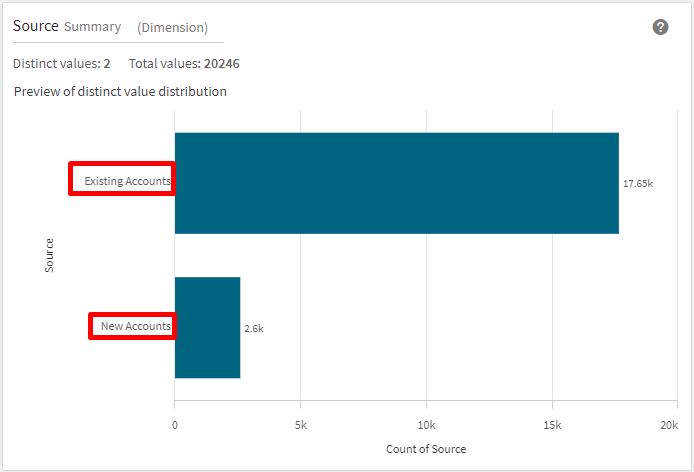
\includegraphics[width=13cm]{./img/img6.5.png}
            \end{center}
        \end{itemize}
    \end{enumerate}
    %%%%%%%%%%%%%%%%%%%%%%%%%%%%%%%%%%%%%%%%%%%%%%%%%%%%%%%%%%%%%%%%%%%%%%%%%%%%%%%%%%%%%%%%%%%%%%%%%%%%%%%%%%%%%%%%%%%%%%%%%%%%%%%%%%%%%%%%%%%%%%%%%%%%%%%%%%%%%%%%%%%%%%%%%%%%%%%%%%%%%%%%%%%%%%%%%%%%%%%%%%%%%%%%%%%%%%%%%%%%%%%%%%%%%%%%%%%%%%%%%%%%%%%%%%%%%%%%%%%%%%%%%%%%%%%%%%%%%%%%%%%%%%%%%%%%%%%%%%%%%%%%%%%%%%%%%%%%%%%%%%%%%%%%%%%%%%%%%%%%%%%%%%%%%%%%%%%%%%%%%%%%%%%%%%%%%%%%%%%%%%%%%%%%%%%%%%%%%%%%%%%%%%%%%%%%%%%%%%%%%%%%%%%%%%%%%%%%%%%%%%%%%%%%%%%%%%%%%%%%%%%%%%%%%%%%%%%%%%%%%%%%%%%%%%%%%%%
    \subsection{Desarrolle una hoja con el ‘Insight advisor’}
    \begin{enumerate}[\tab 1.]
        \item Use el submenú de navegación de acceso rápido en \textit{Analize} $>$ \textbf{Sheet} para seleccionar \textbf{Insights}.
        \begin{center}
            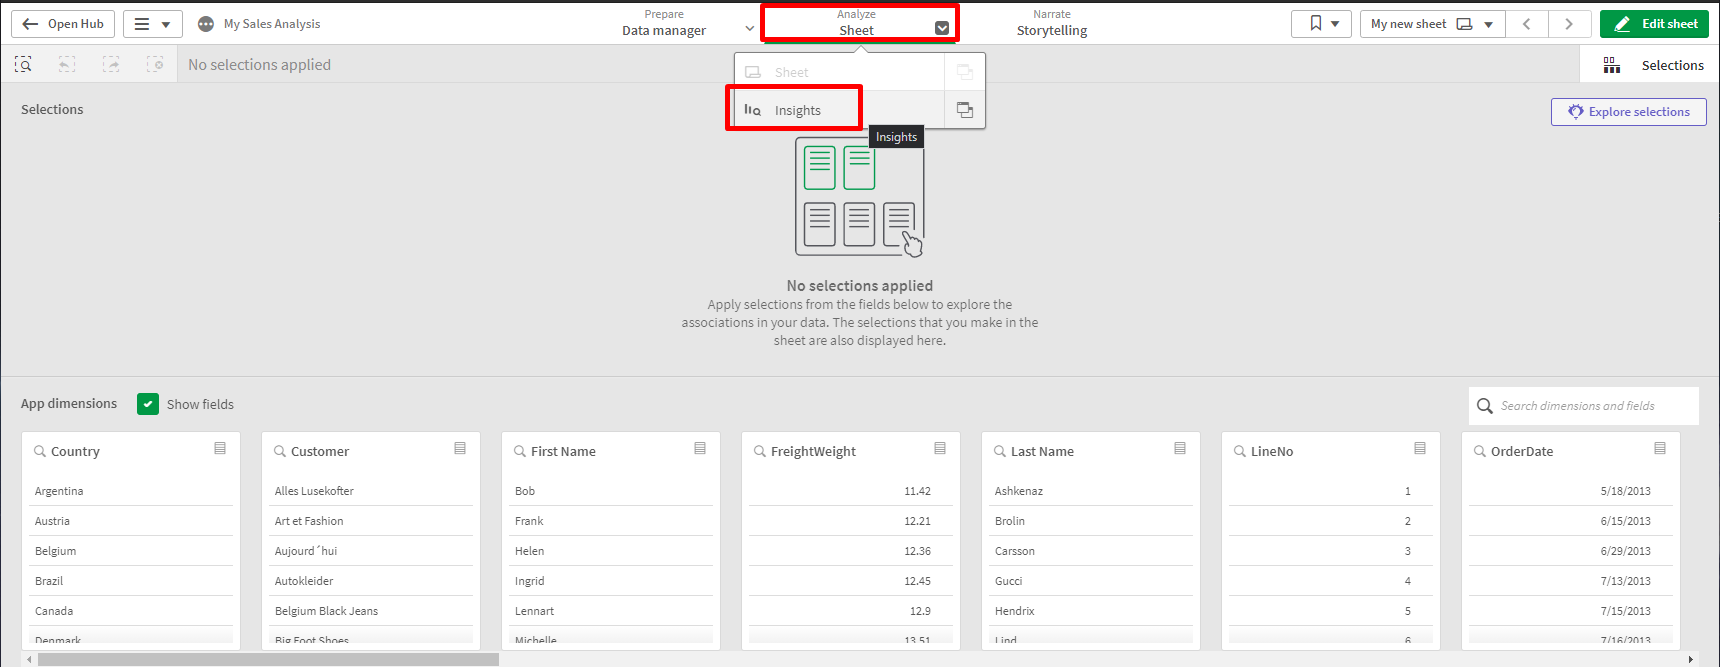
\includegraphics[width=13cm]{./img/img7.png}
        \end{center}
        \item Haga clic en el botón para \textbf{Generar insights}, basado en todo el modelo de datos.
        \begin{center}
            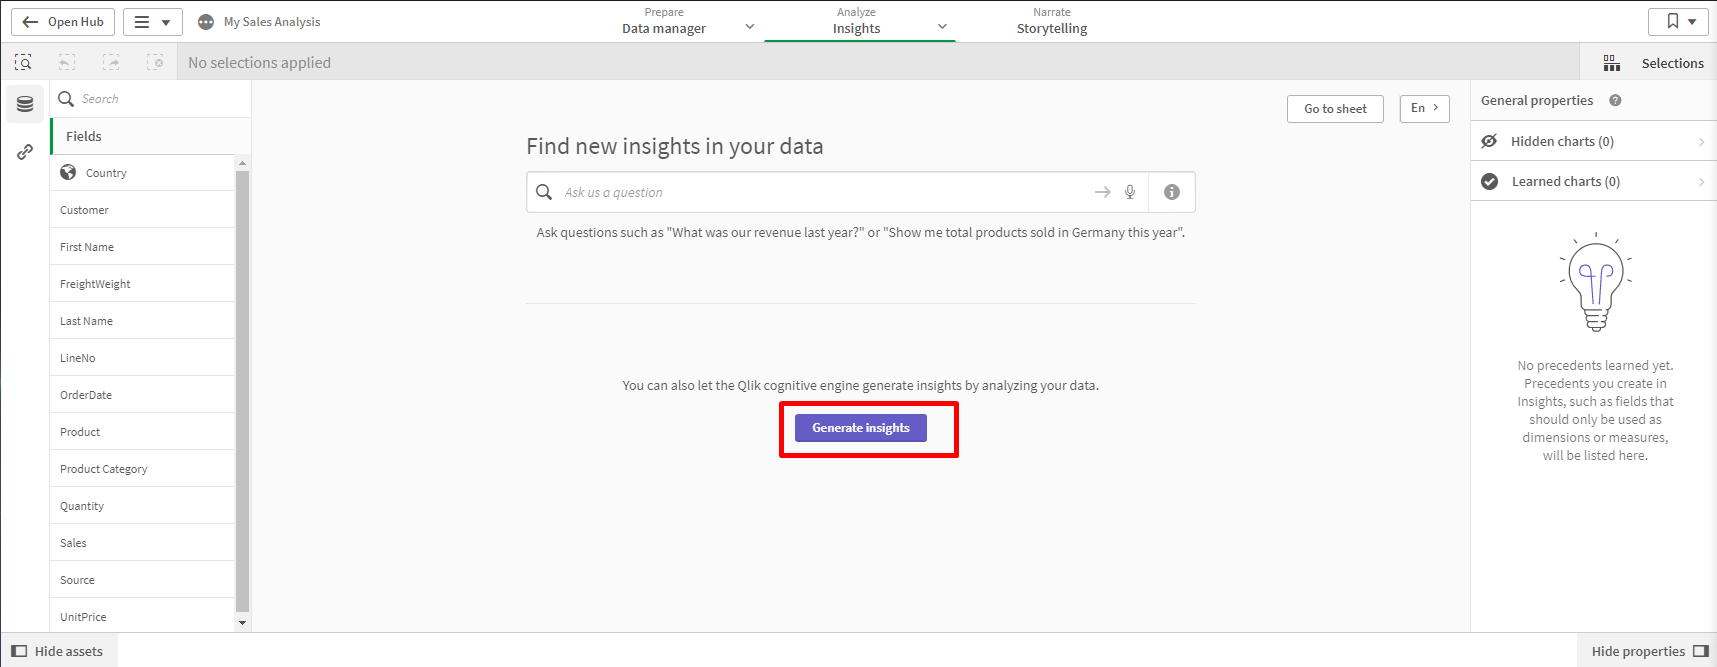
\includegraphics[width=13cm]{./img/img8.png}
        \end{center}
        \item Busque el mapa en la lista de gráficos propuestos y seleccione \textbf{Add to sheet} $>$ \textit{My new sheet}.
        \begin{center}
            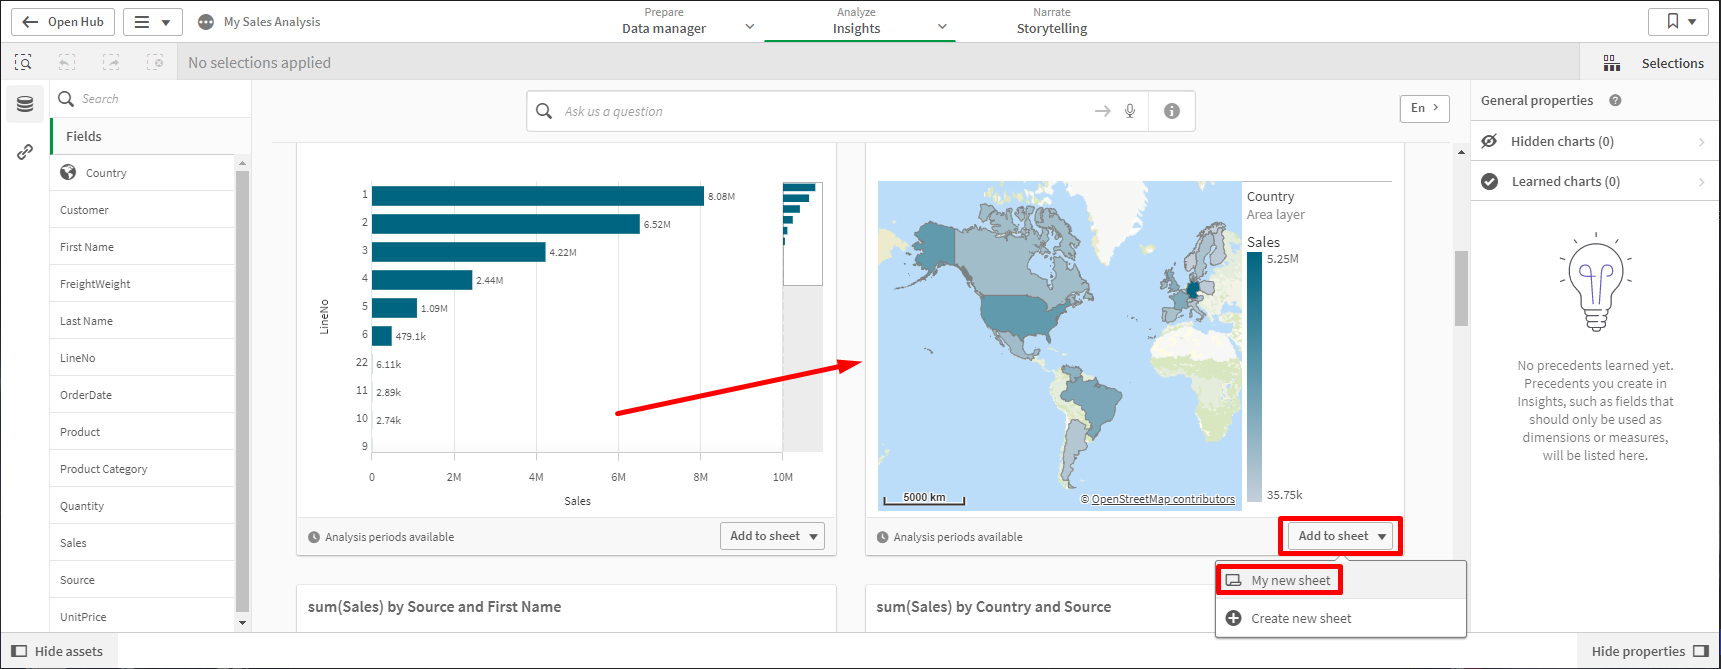
\includegraphics[width=13cm]{./img/img9.png}
        \end{center}
        \item Utilice el panel de la izquierda para seleccionar (casillas marcadas) los campos: \textit{Product} y \textit{UnitPrice}.
        \begin{center}
            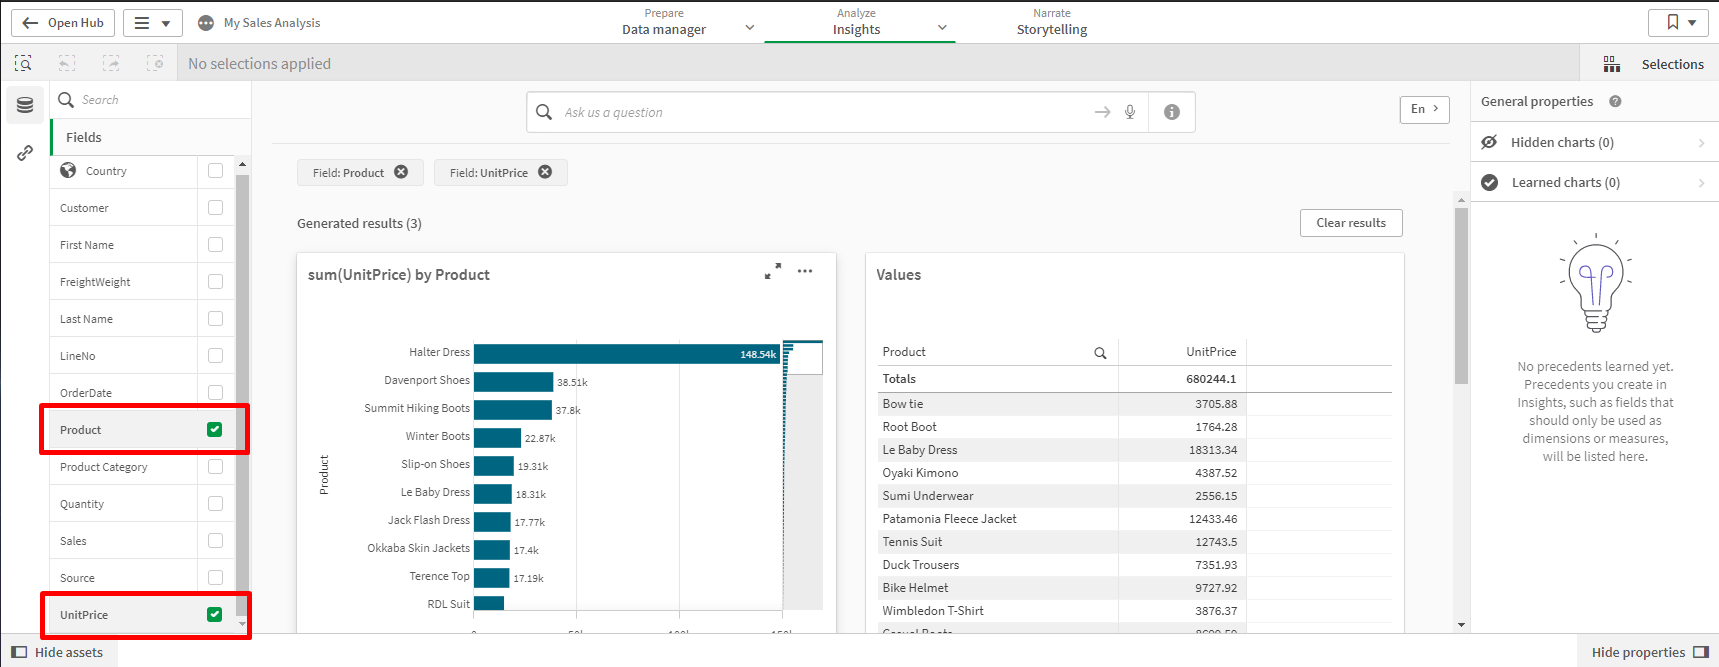
\includegraphics[width=13cm]{./img/img10.png}
        \end{center}
        \begin{itemize}
            \item Busque el gráfico de barras titulado: \textit{sum(UnitPrice) by Product} y sleccione \textbf{Add to sheet} $>$  \textit{My new sheet}.
            \begin{center}
                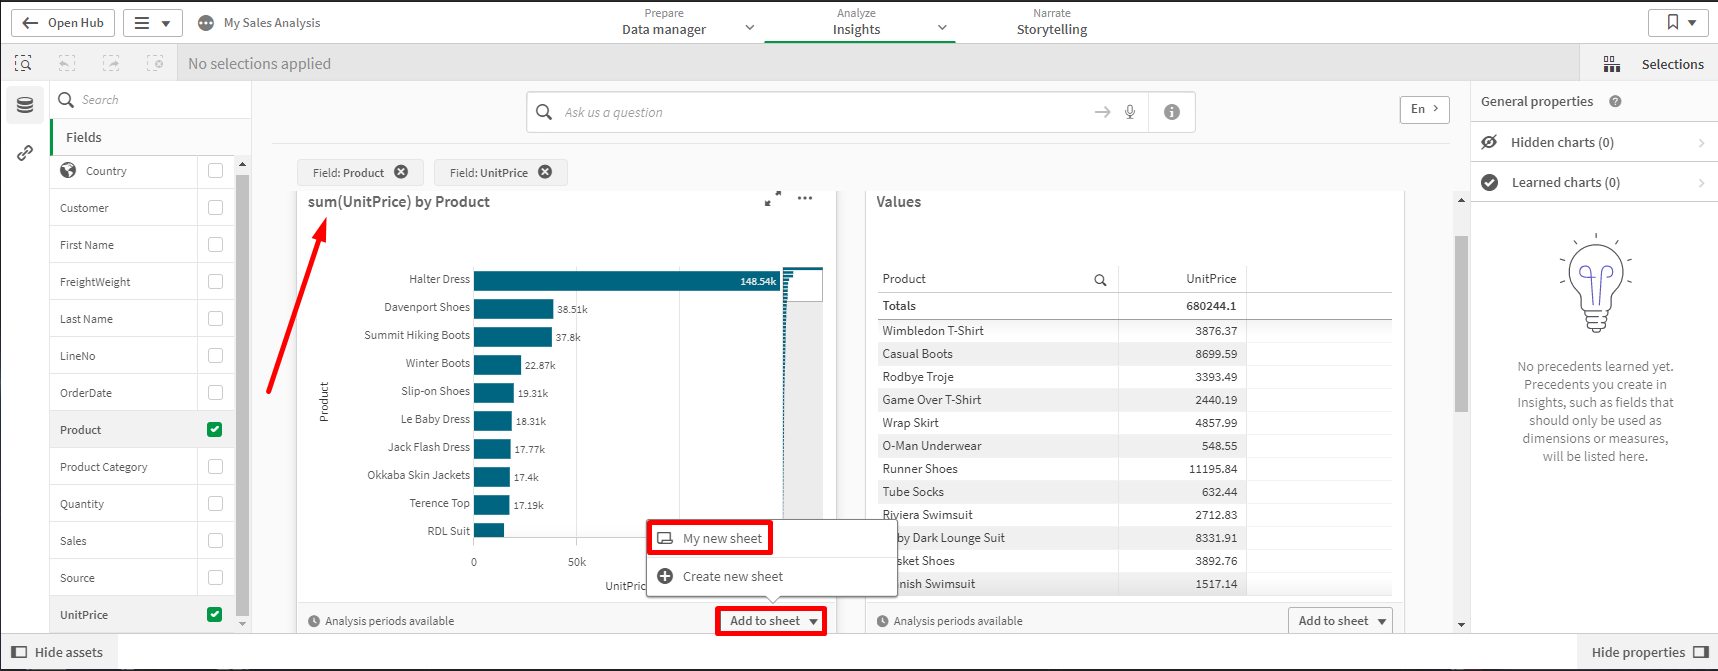
\includegraphics[width=13cm]{./img/img10.1.png}
            \end{center}
            \item Podemos limpiar los filtros haciendo clic en la \textit{\textbf{'x'}}.
            \begin{center}
                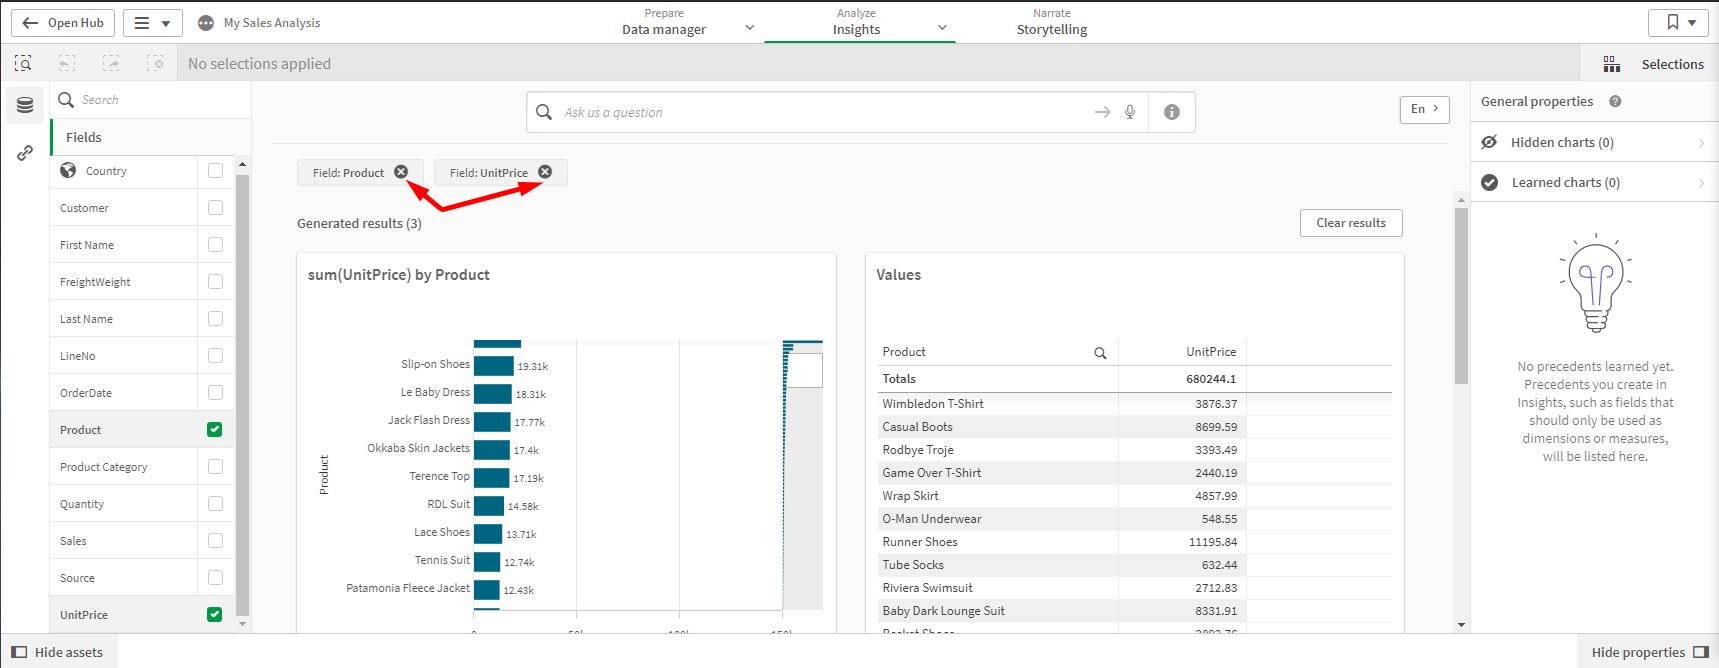
\includegraphics[width=13cm]{./img/img10.2.png}
            \end{center}
        \end{itemize}
        \item Escriba lo siguiente en el campo \textit{‘Ask us a question’}: \textbf{Which country has highest quantity?} (y enviar pregunta).
        \begin{center}
            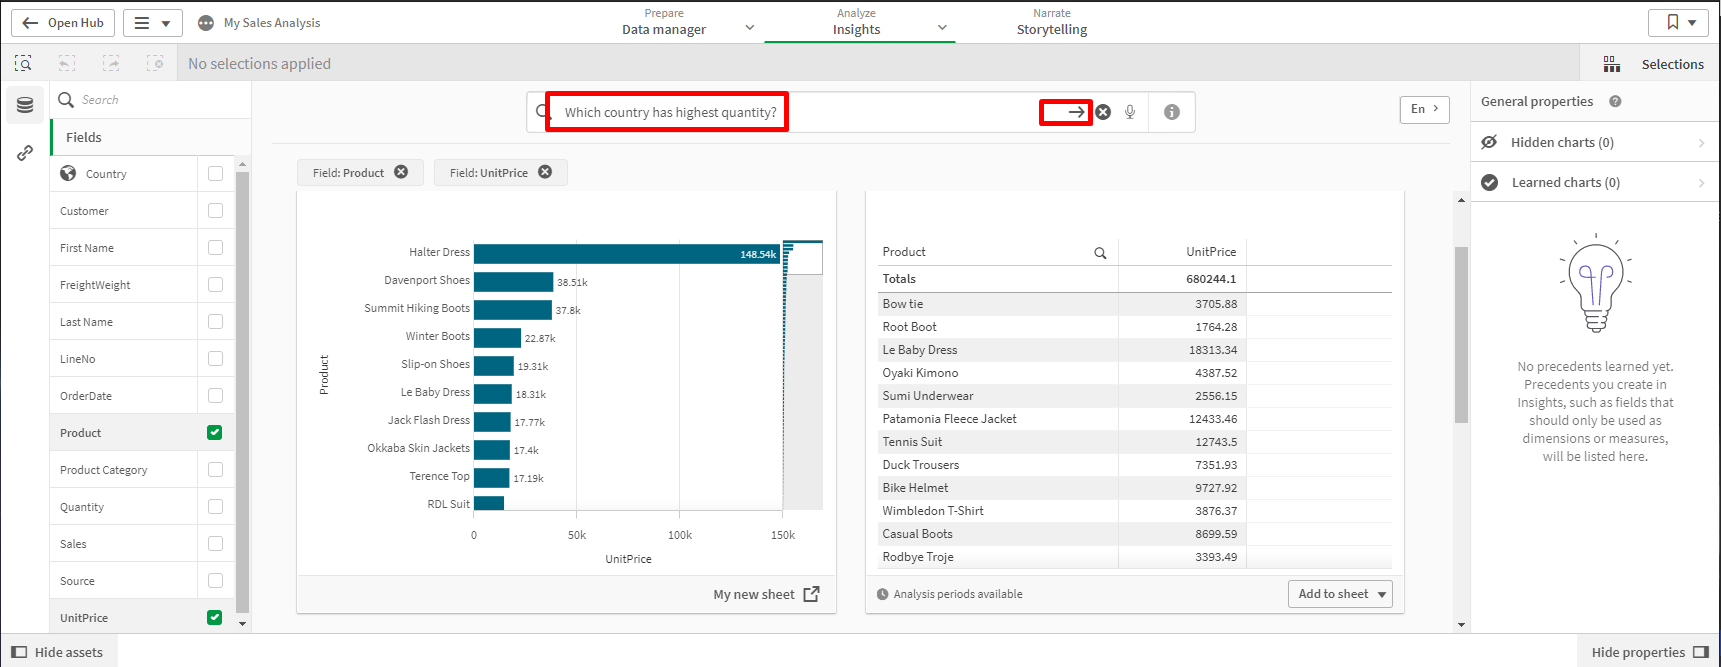
\includegraphics[width=13cm]{./img/img11.png}
        \end{center}
        \begin{itemize}
            \item Busque el gráfico de barras titulado: \textit{sum(Quantity) by Country} y seleccione \textbf{Add to sheet} $>$ \textbf{My new sheet}.
            \begin{center}
                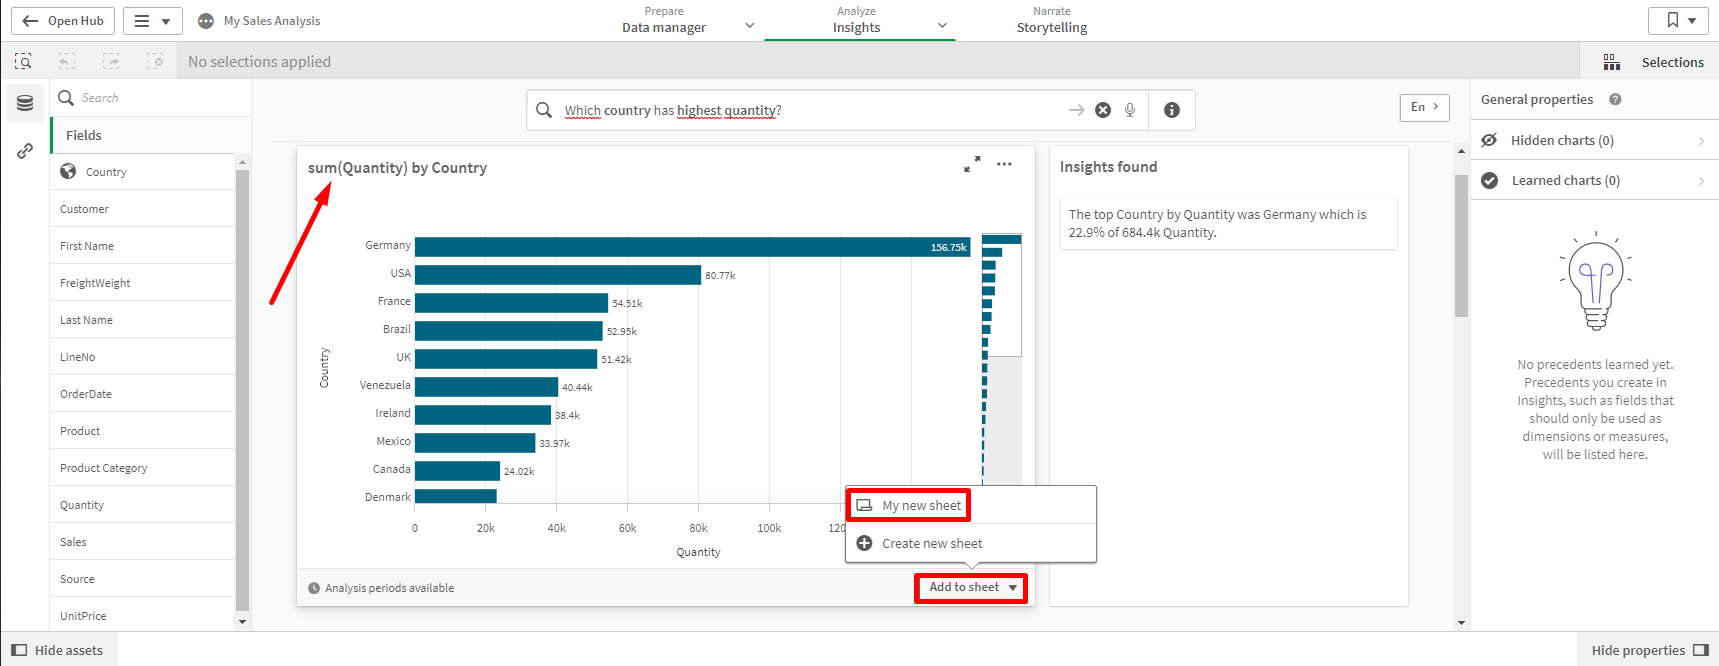
\includegraphics[width=13cm]{./img/img11.1.png}
            \end{center}
        \end{itemize}
        \item Utilice el submenú de navegación de acceso rápido en \textit{Analyze} $>$ \textbf{Insights} para seleccionar \textbf{Sheet}.
        \begin{center}
            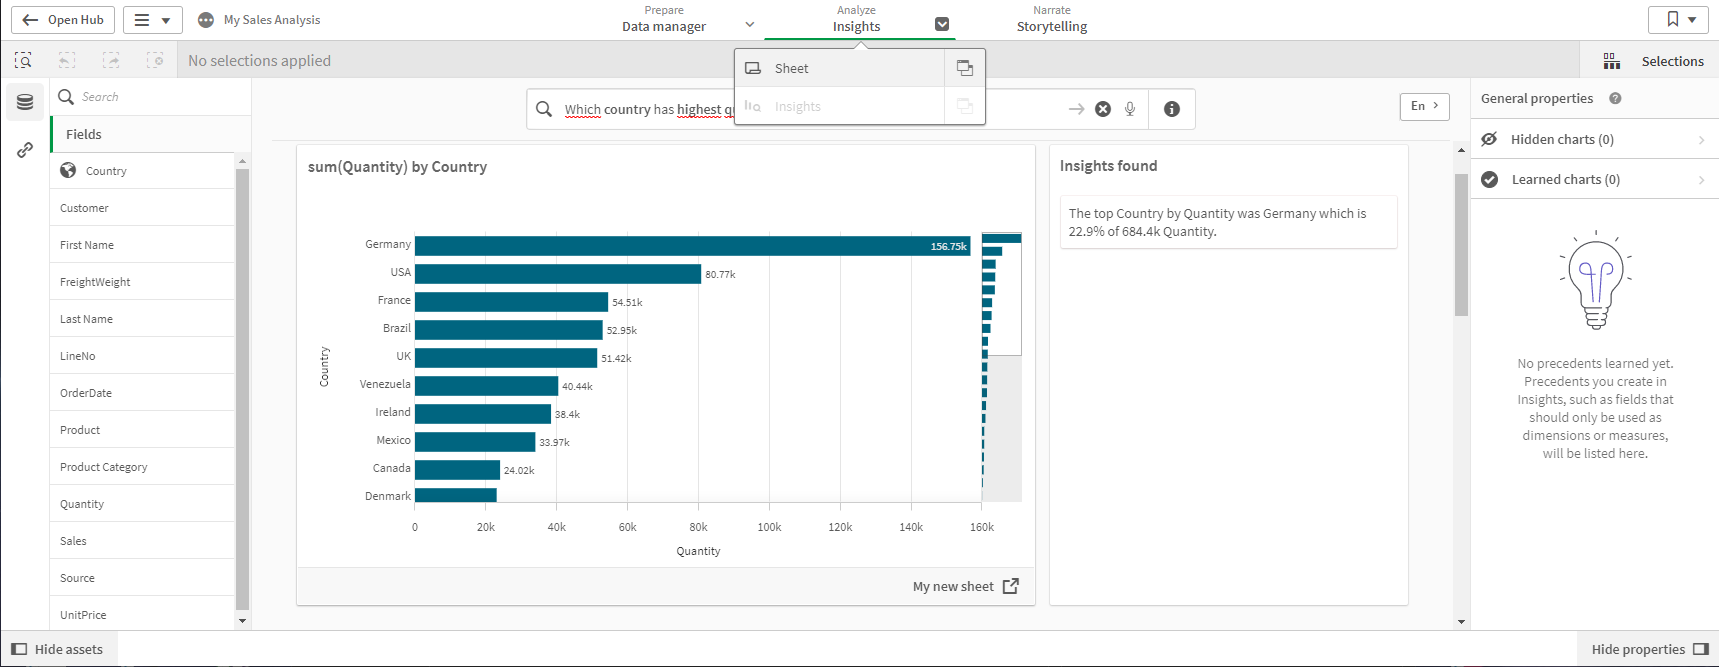
\includegraphics[width=13cm]{./img/img12.png}
        \end{center}
        \item Evaluar la hoja que ha creado. Debería aparecer como ve a continuación:
        \begin{center}
            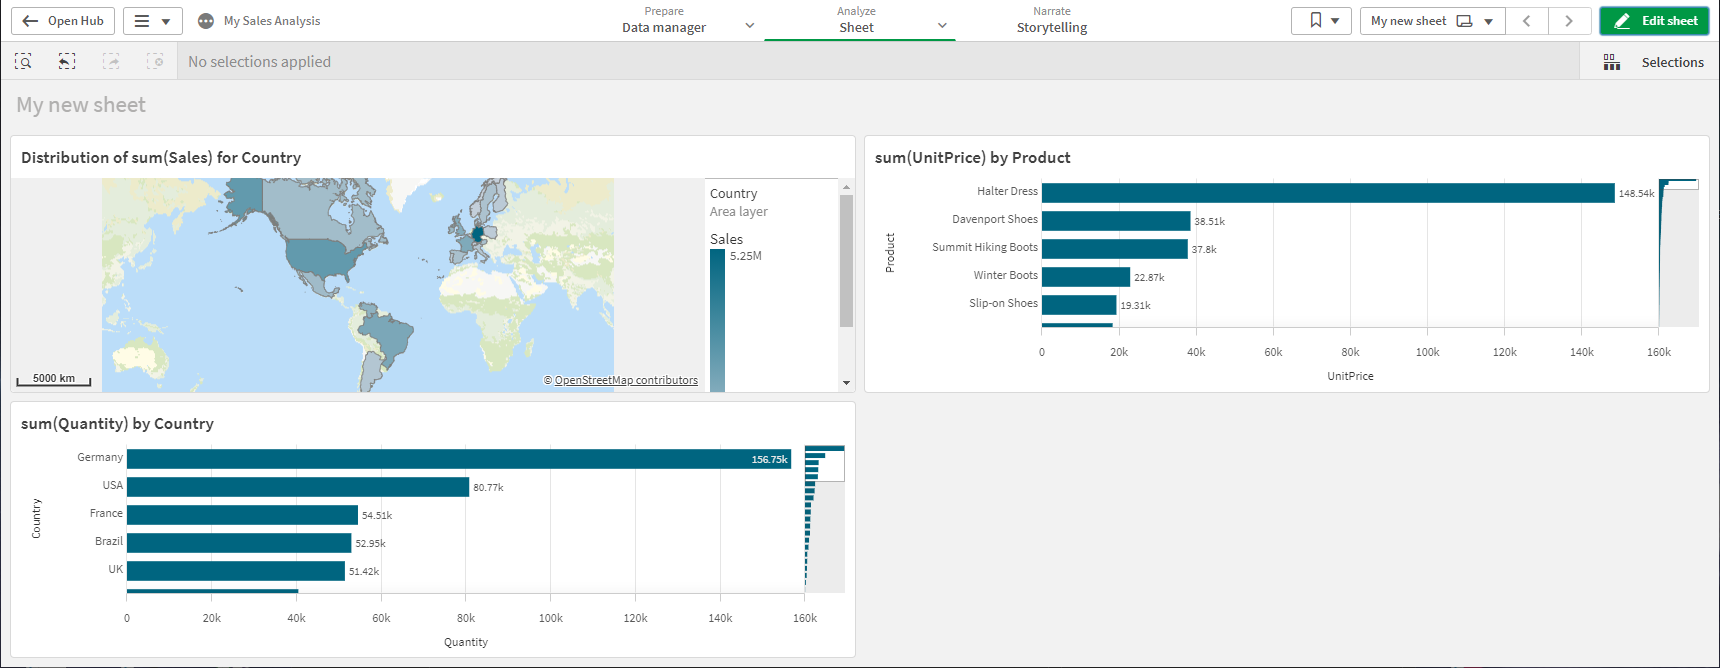
\includegraphics[width=13cm]{./img/img13.png}
        \end{center}
        \item Cambie la hoja al modo de \textbf{Edición} (el lapiz) y use el panel de propiedades para cambiar el título de la hoja.
        \begin{center}
            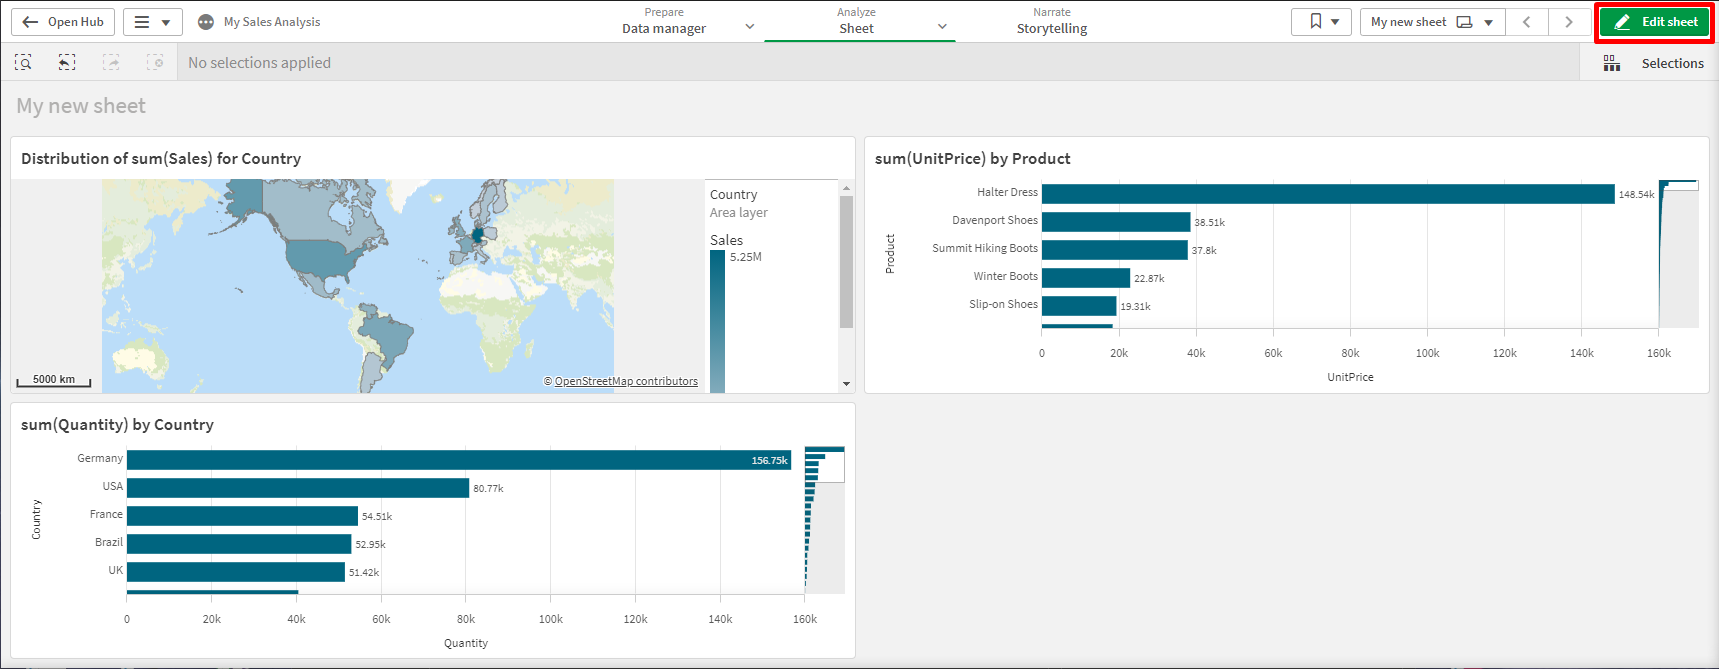
\includegraphics[width=13cm]{./img/img14.png}
        \end{center}
        \item Cambiar el título de la hoja de \textit{\textbf{“My new sheet”}} a \textit{\textbf{“My insights”}} y para terminar la edicion  clic en el boton \textbf{"Done editing"}.
        \begin{center}
            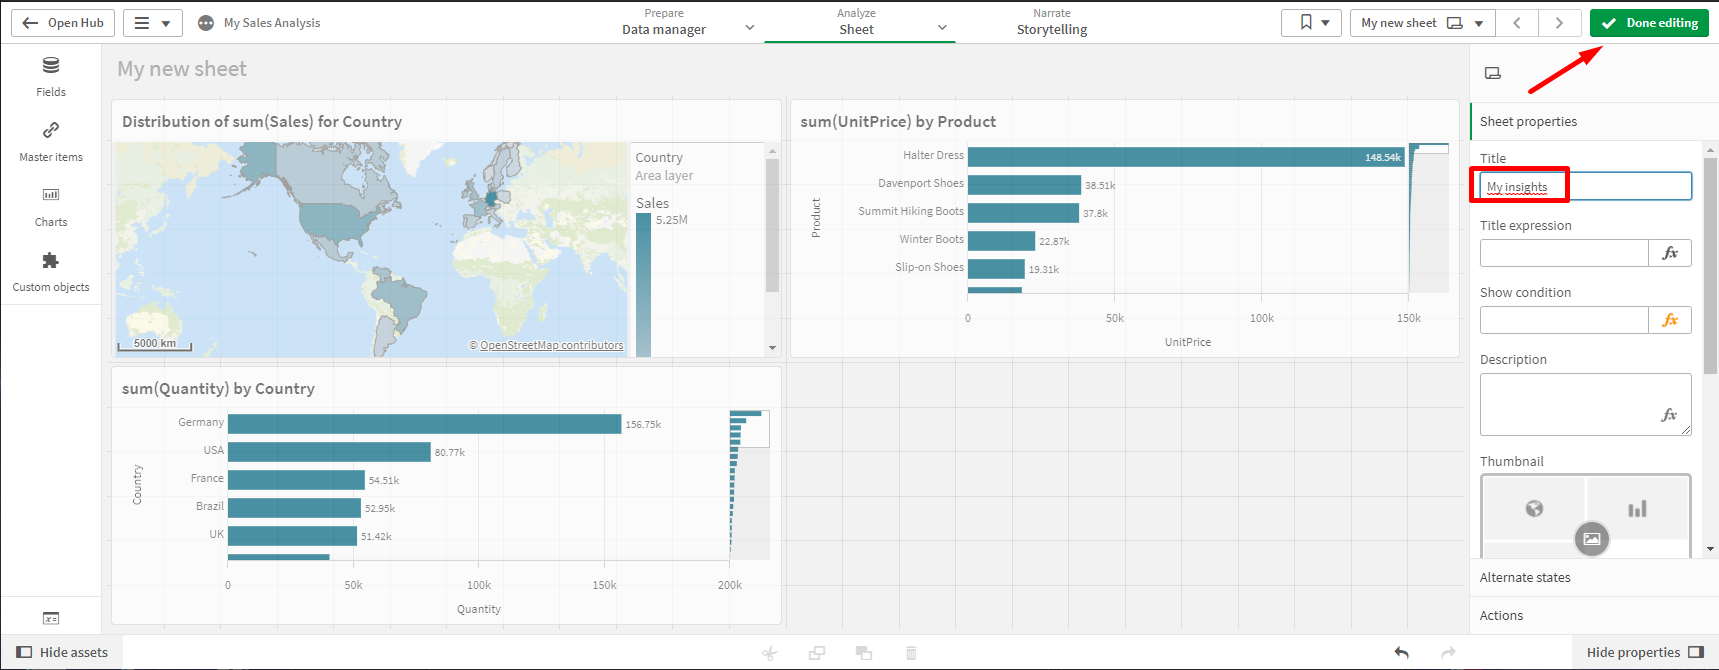
\includegraphics[width=13cm]{./img/img15.png}
        \end{center}
    \end{enumerate}
    %%%%%%%%%%%%%%%%%%%%%%%%%%%%%%%%%%%%%%%%%%%%%%%%%%%%%%%%%%%%%%%%%%%%%%%%%%%%%%%%%%%%%%%%%%%%%%%%%%%%%%%%%%%%%%%%%%%%%%%%%%%%%%%%%%%%%%%%%%%%%%%%%%%%%%%%%%%%%%%%%%%%%%%%%%%%%%%%%%%%%%%%%%%%%%%%%%%%%%%%%%%%%%%%%%%%%%%%%%%%%%%%%%%%%%%%%%%%%%%%%%%%%%%%%%%%%%%%%%%%%%%%%%%%%%%%%%%%%%%%%%%%%%%%%%%%%%%%%%%%%%%%%%%%%%%%%%%%%%%%%%%%%%%%%%%%%%%%%%%%%%%%%%%%%%%%%%%%%%%%%%%%%%%%%%%%%%%%%%%%%%%%%%%%%%%%%%%%%%%%%%%%%%%%%%%%%%%%%%%%%%%%%%%%%%%%%%%%%%%%%%%%%%%%%%%%%%%%%%%%%%%%%%%%%%%%%%%%%%%%%%%%%%%%%%%%%%%
    \subsection{Desarrolle una hoja utilizando ‘Chart suggestion assistance’}
    \begin{enumerate}[\tab 1.]
        \item Utilice el menú desplegable de hojas (icono de hoja) para crear una nueva hoja.
        \begin{center}
            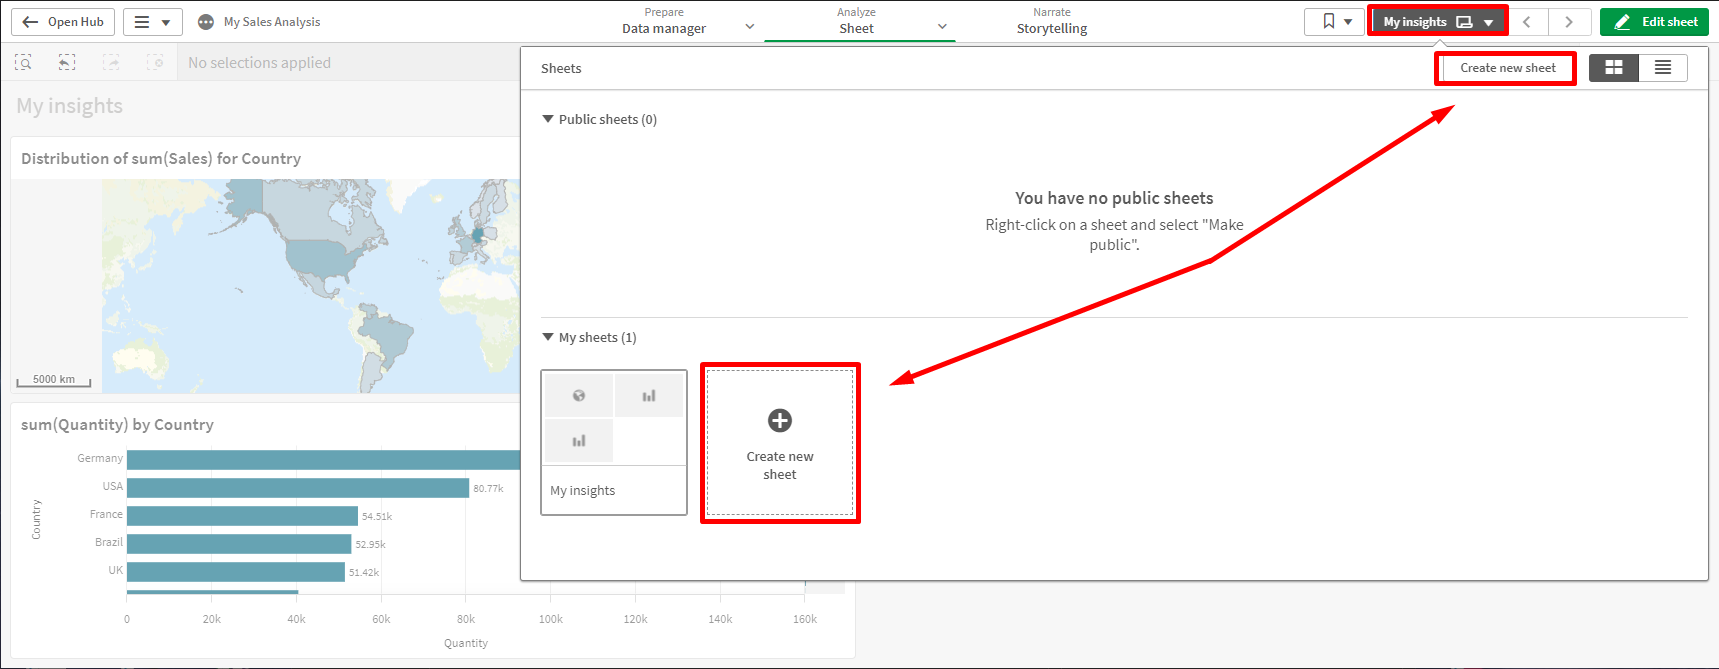
\includegraphics[width=13cm]{./img/img16.png}
        \end{center}
        \begin{itemize}
            \item Coloquele de titulo a la hoja: \textit{\textbf{“My suggestions“}}.
            \begin{center}
                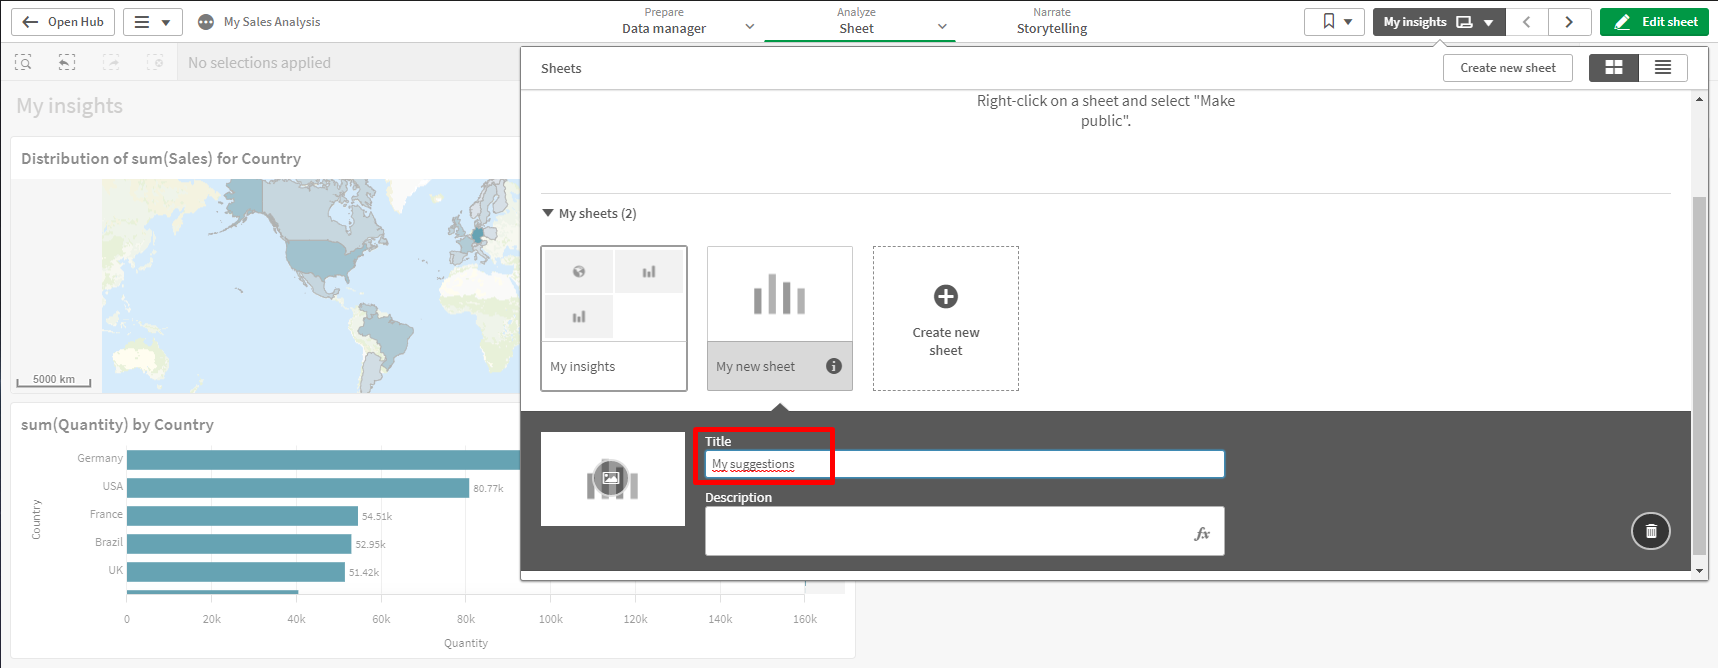
\includegraphics[width=13cm]{./img/img16.1.png}
            \end{center}
        \end{itemize}
        \item En el modo Editar hoja, use la sección Campos (icono de BD) del panel de activos, arrastre y suelte el campo \textit{\textbf{Sales}} en el área de visualización.
        \begin{center}
            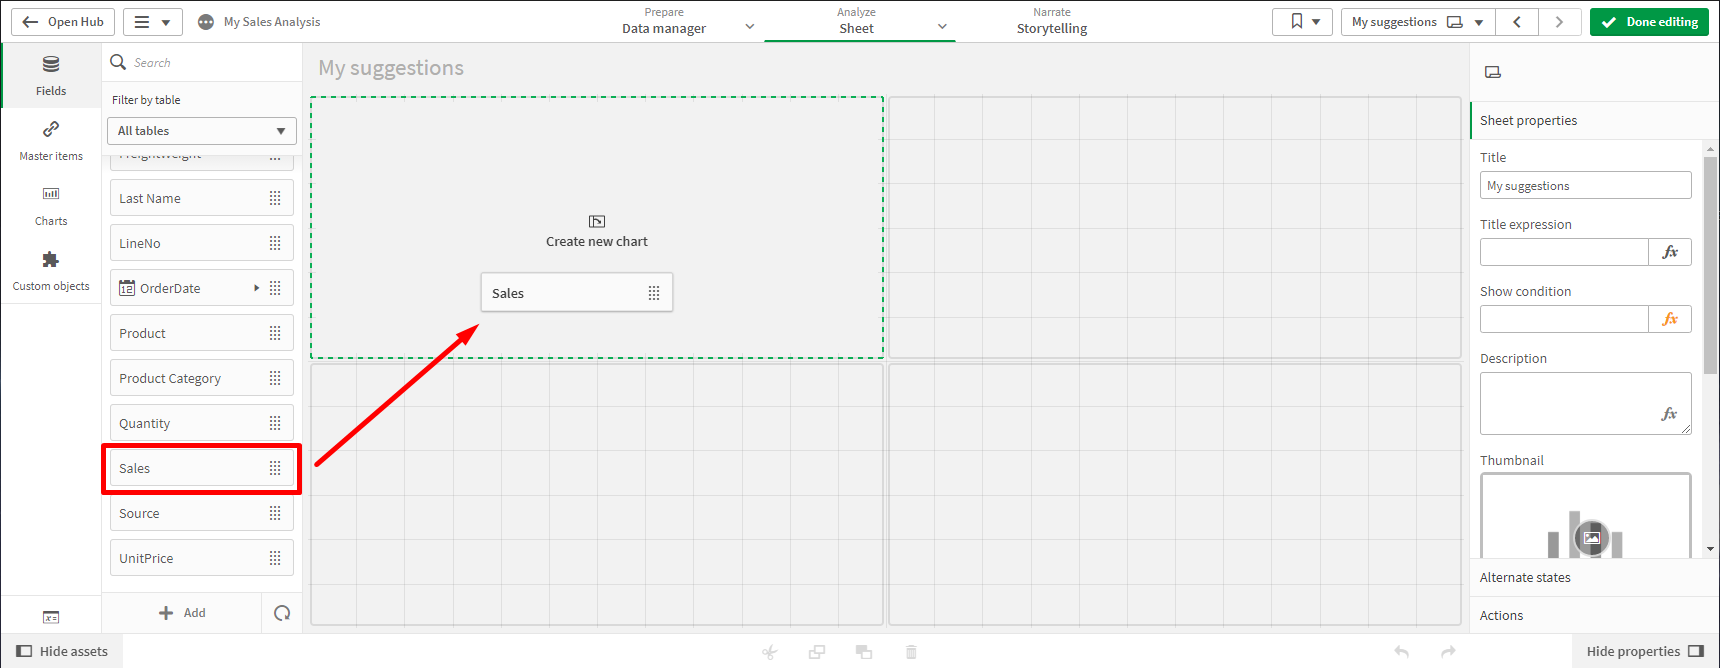
\includegraphics[width=13cm]{./img/img17.png}
        \end{center}
        \begin{itemize}
            \item Se obtiene un tipo de gráfico de KPI, que muestra la suma de los valores de ventas para todo el modelo de datos.
            \begin{center}
                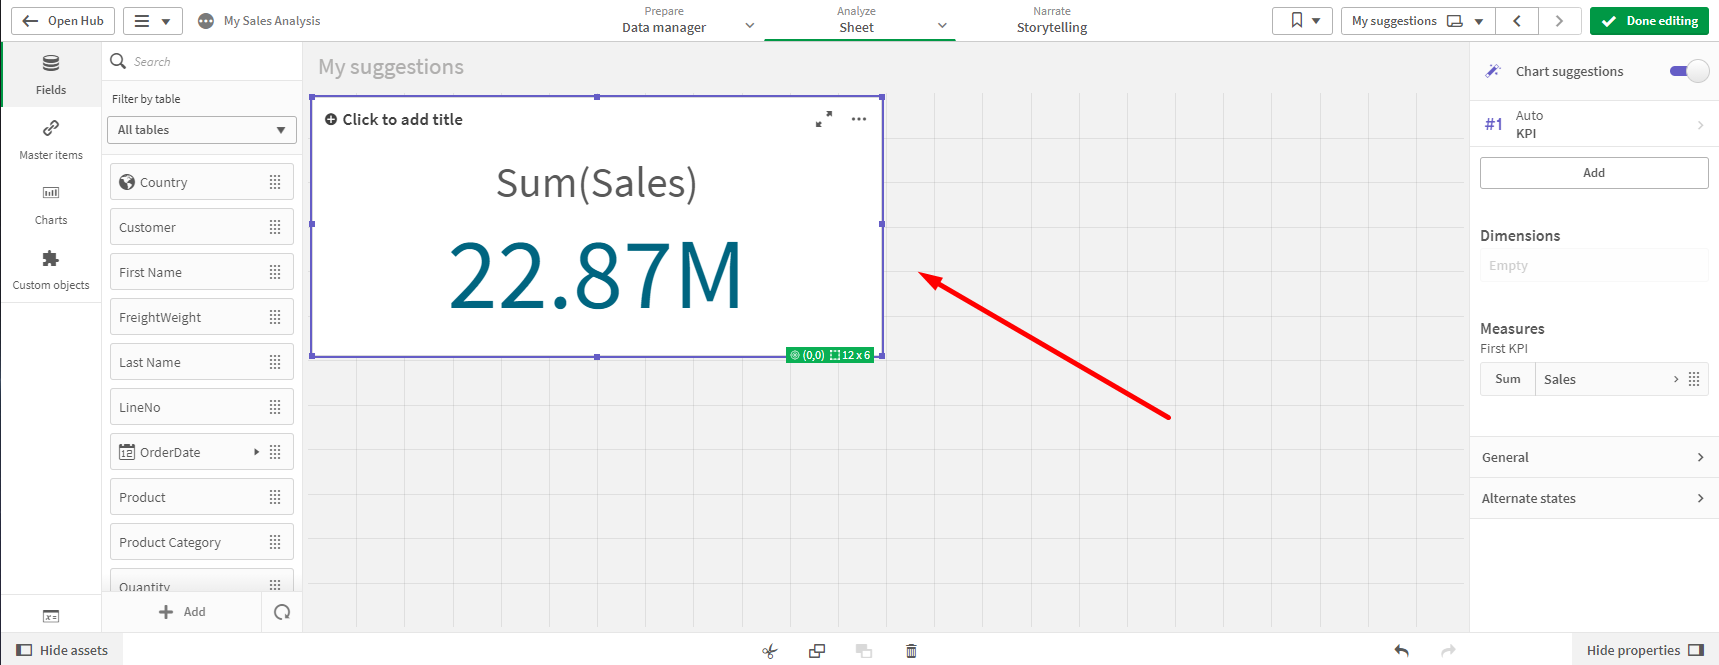
\includegraphics[width=13cm]{./img/img17.1.png}
            \end{center}
            \item Además, el interruptor de \textit{\textbf{Sugerencias de Gráficos}} en la parte superior del panel de propiedades está "activado".
            \begin{center}
                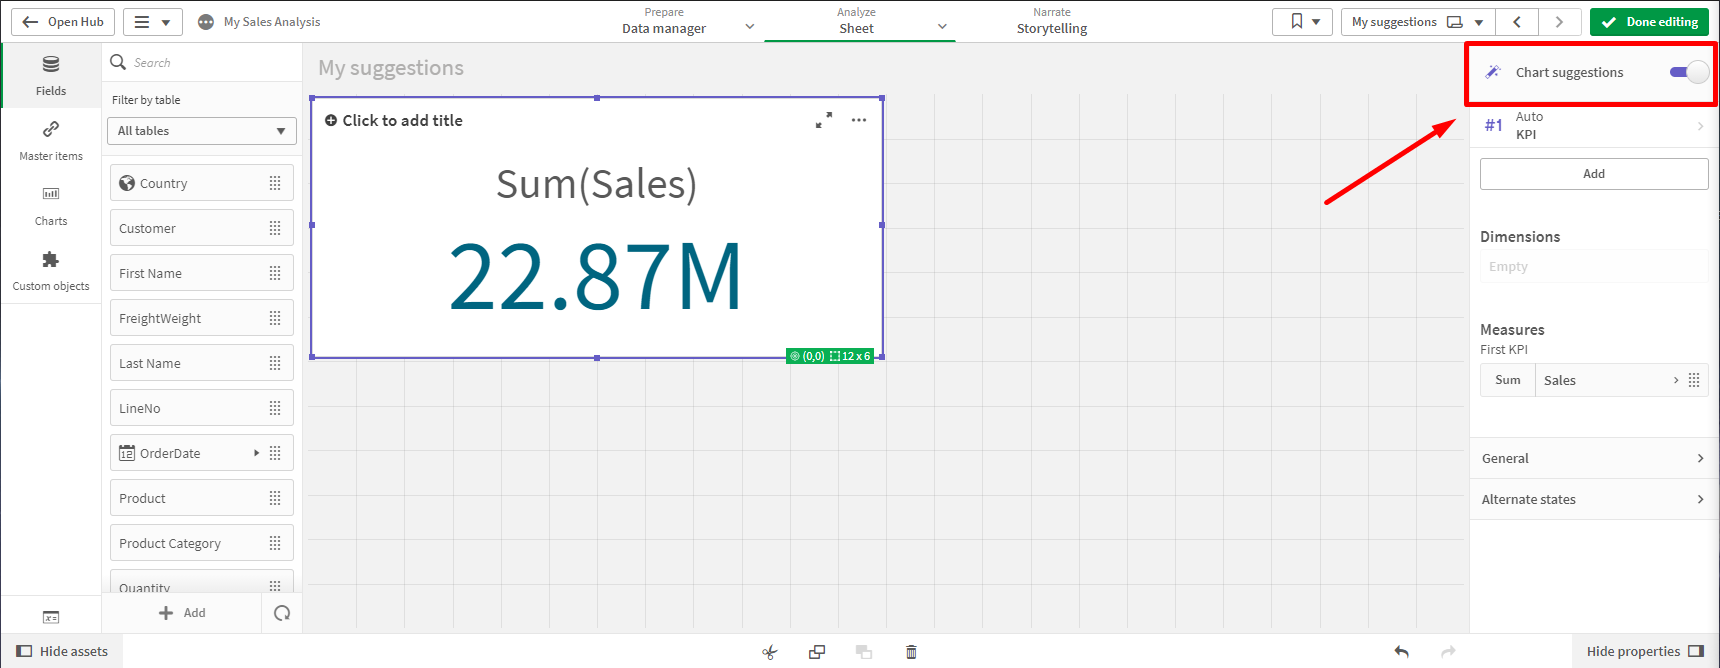
\includegraphics[width=13cm]{./img/img17.2.png}
            \end{center}
        \end{itemize}
        \item Arrastre y suelte el campo \textit{Country} en el gráfico de KPI, asegurándose de que la imagen "fantasma" cubra todo el gráfico.
        \begin{center}
            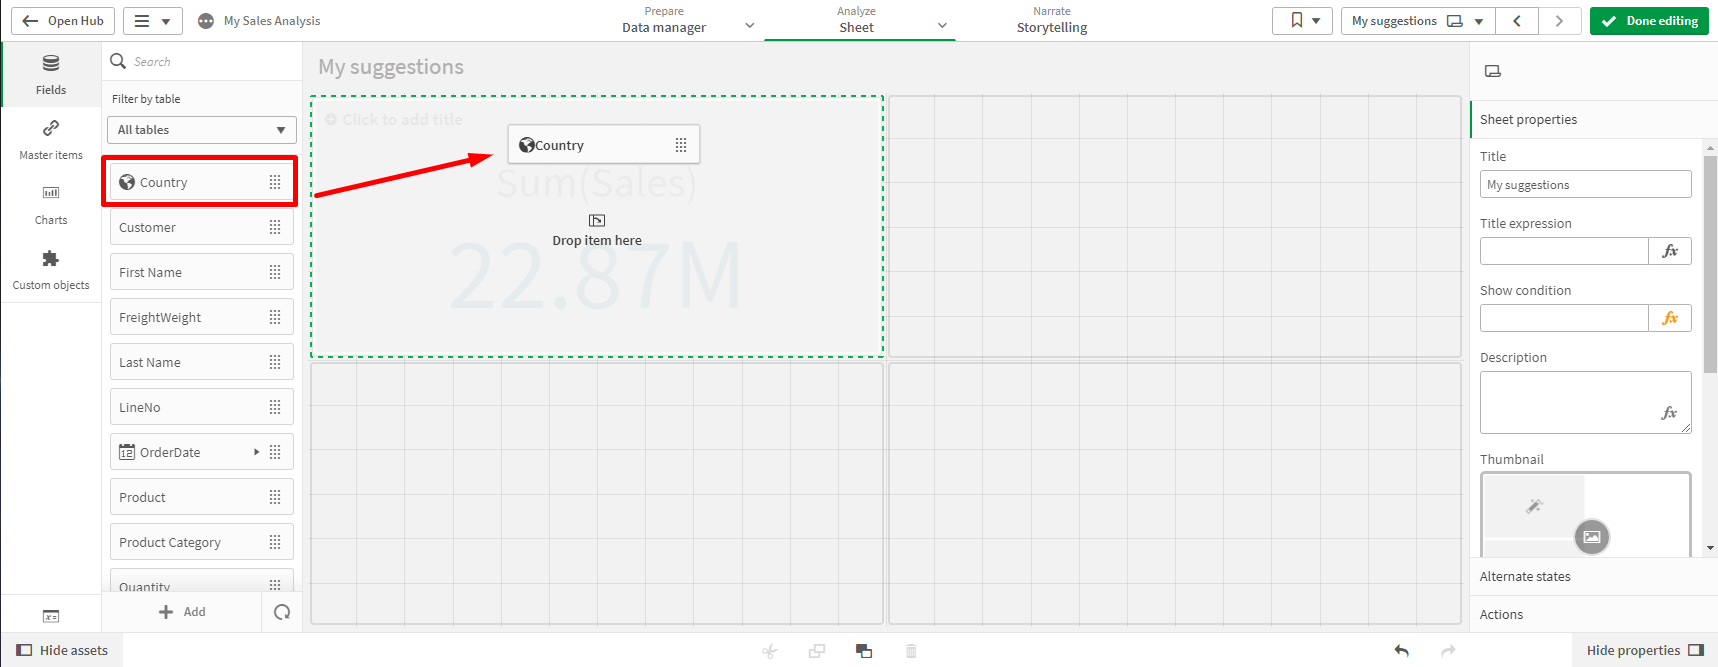
\includegraphics[width=13cm]{./img/img18.png}
        \end{center}
        \begin{itemize}
            \item Se obtiene un tipo de gráfico de mapa y el color del mapa relaciona la suma de los valores de ventas en cada país.
            \begin{center}
                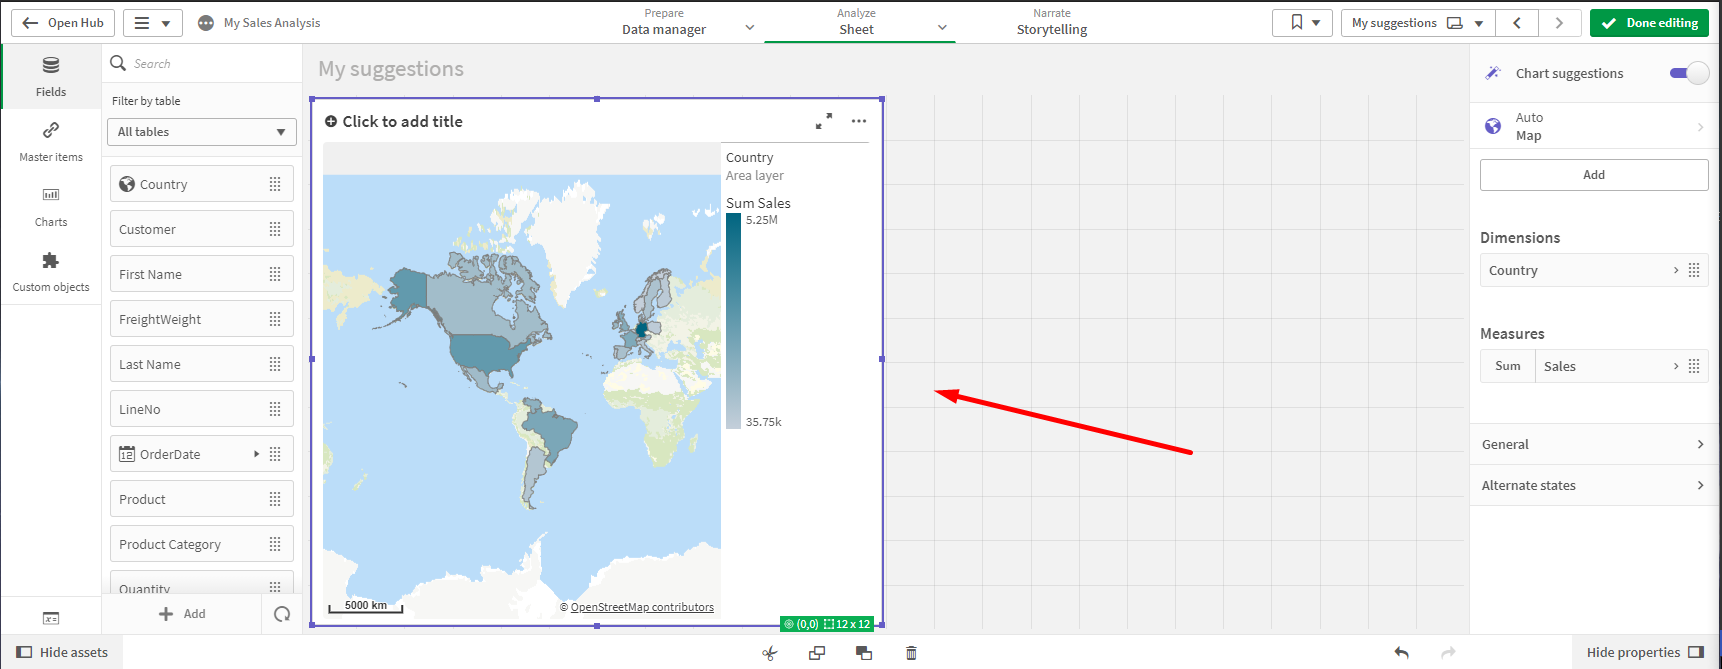
\includegraphics[width=13cm]{./img/img18.1.png}
            \end{center}
        \end{itemize}
    \end{enumerate}
    %%%%%%%%%%%%%%%%%%%%%%%%%%%%%%%%%%%%%%%%%%%%%%%%%%%%%%%%%%%%%%%%%%%%%%%%%%%%%%%%%%%%%%%%%%%%%%%%%%%%%%%%%%%%%%%%%%%%%%%%%%%%%%%%%%%%%%%%%%%%%%%%%%%%%%%%%%%%%%%%%%%%%%%%%%%%%%%%%%%%%%%%%%%%%%%%%%%%%%%%%%%%%%%%%%%%%%%%%%%%%%%%%%%%%%%%%%%%%%%%%%%%%%%%%%%%%%%%%%%%%%%%%%%%%%%%%%%%%%%%%%%%%%%%%%%%%%%%%%%%%%%%%%%%%%%%%%%%%%%%%%%%%%%%%%%%%%%%%%%%%%%%%%%%%%%%%%%%%%%%%%%%%%%%%%%%%%%%%%%%%%%%%%%%%%%%%%%%%%%%%%%%%%%%%%%%%%%%%%%%%%%%%%%%%%%%%%%%%%%%%%%%%%%%%%%%%%%%%%%%%%%%%%%%%%%%%%%%%%%%%%%%%%%%%%%%%%%
    \subsection{Desarrolle una hoja usando ‘Chart suggestion assistance’ (cont’d)}
    \begin{enumerate}[\tab 1.]
        \item Expanda el campo \textit{OrderDate} en el panel de activos para exponer agrupaciones de fechas derivadas.
        \begin{center}
            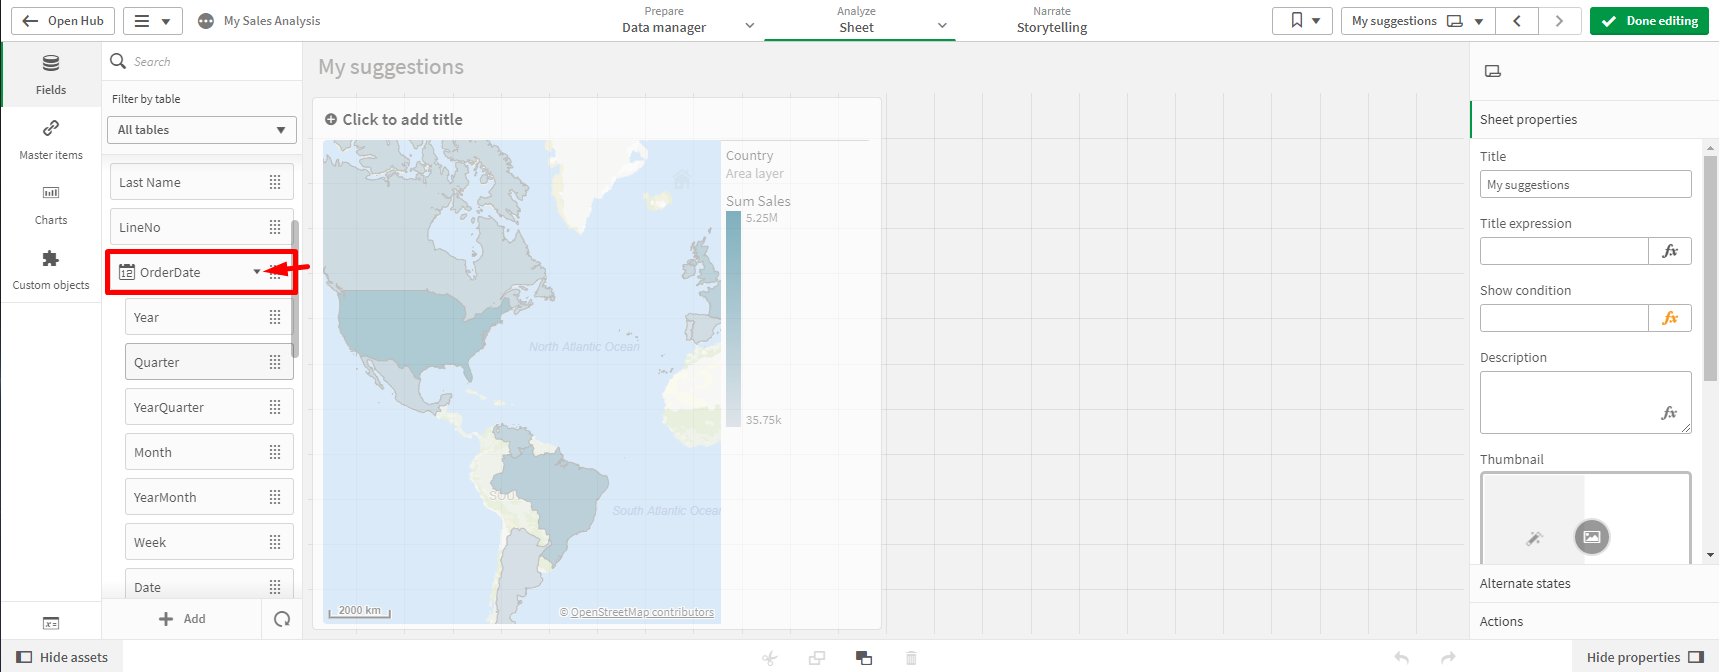
\includegraphics[width=13cm]{./img/img19.png}
        \end{center}
        \begin{itemize}
            \item Arrastre y suelte la agrupación \textit{YearMonth} en un espacio vacío en el área de visualización.
            \begin{center}
                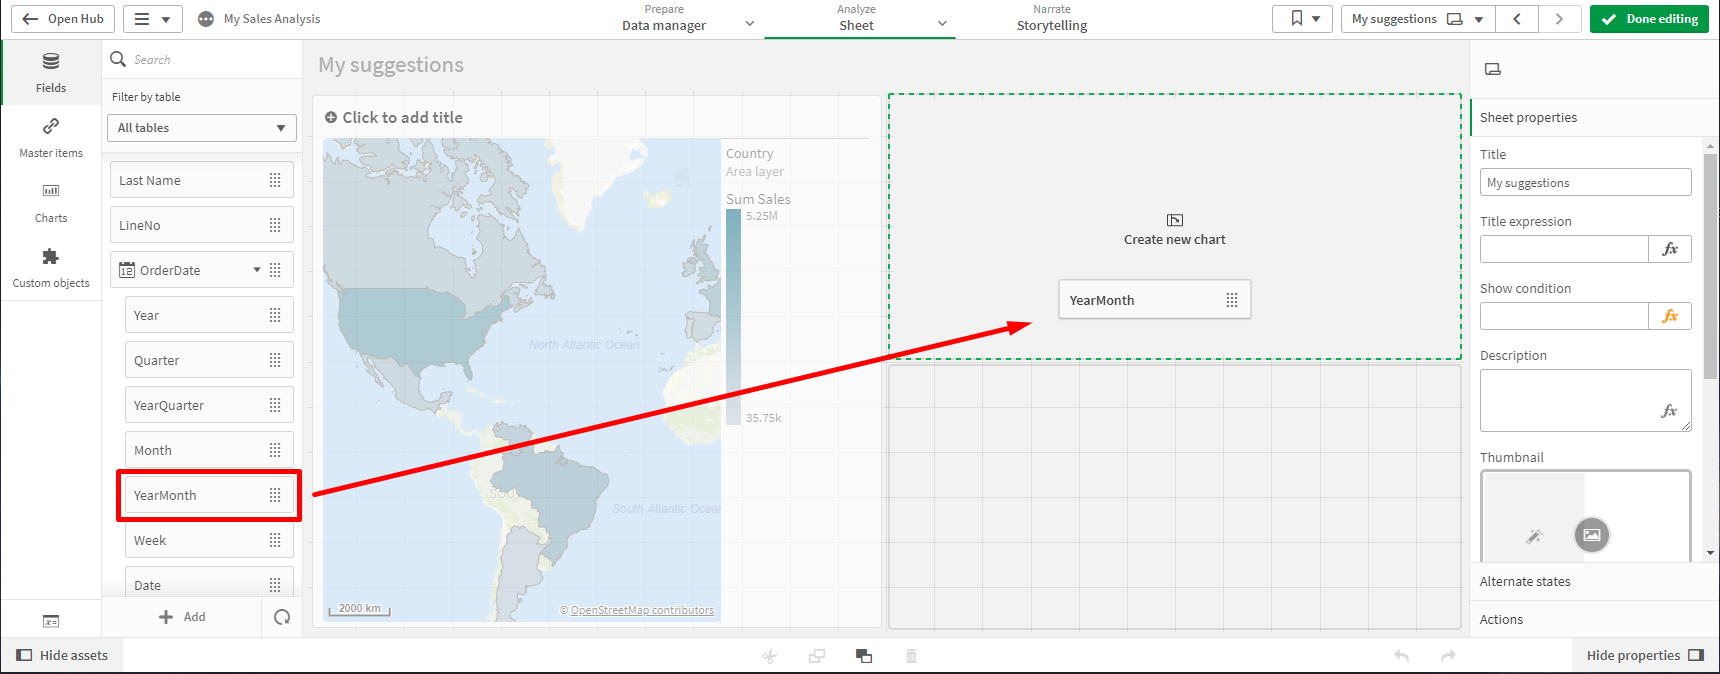
\includegraphics[width=13cm]{./img/img19.1.png}
            \end{center}
            \item Se obtiene un tipo de gráfico de tabla.
            \begin{center}
                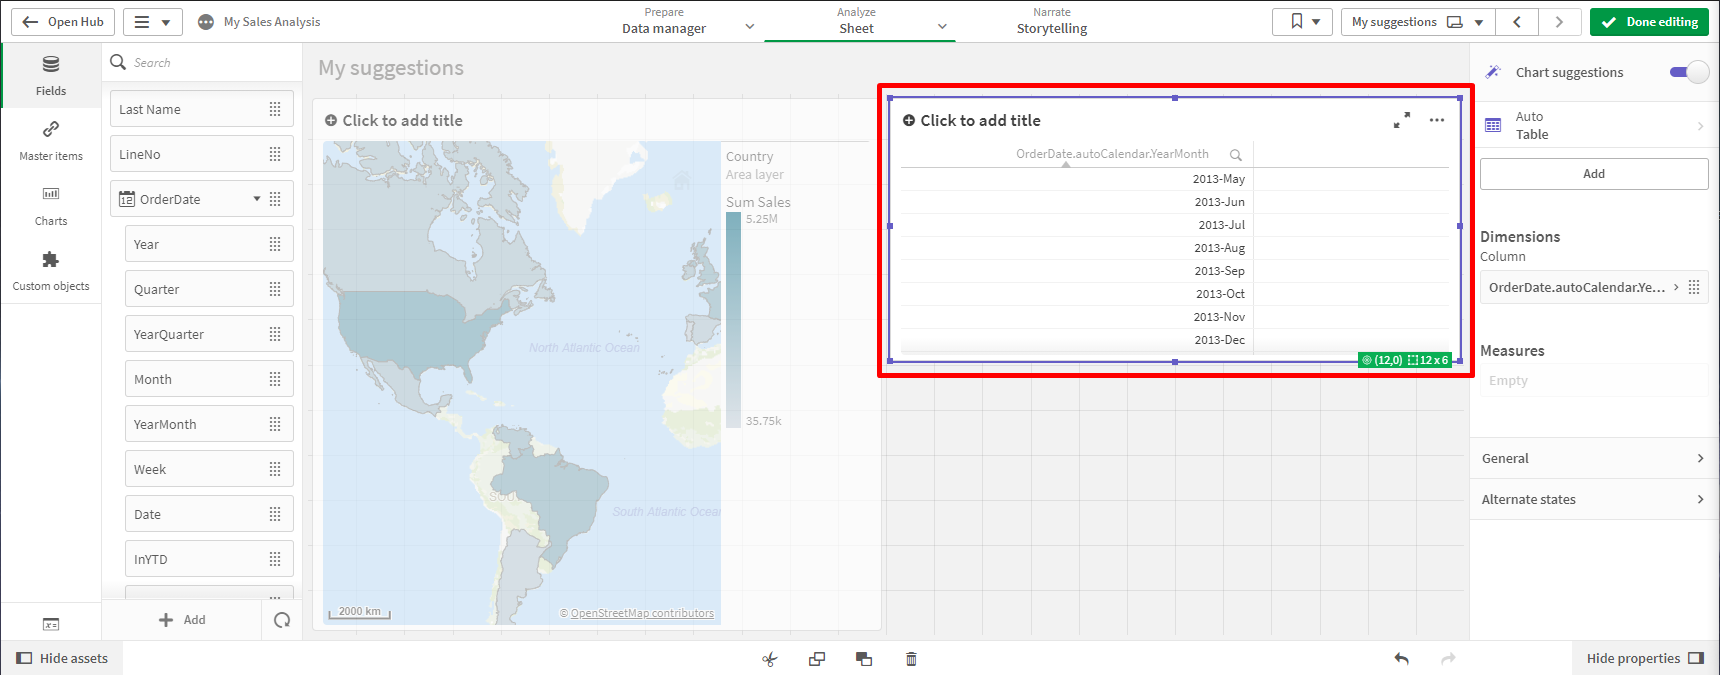
\includegraphics[width=13cm]{./img/img19.2.png}
            \end{center}
        \end{itemize}
        \item Arrastre y suelte el campo \textit{Sales} para cubrir toda la tabla que actualmente muestra los valores de año y mes para los pedidos.
        \begin{center}
            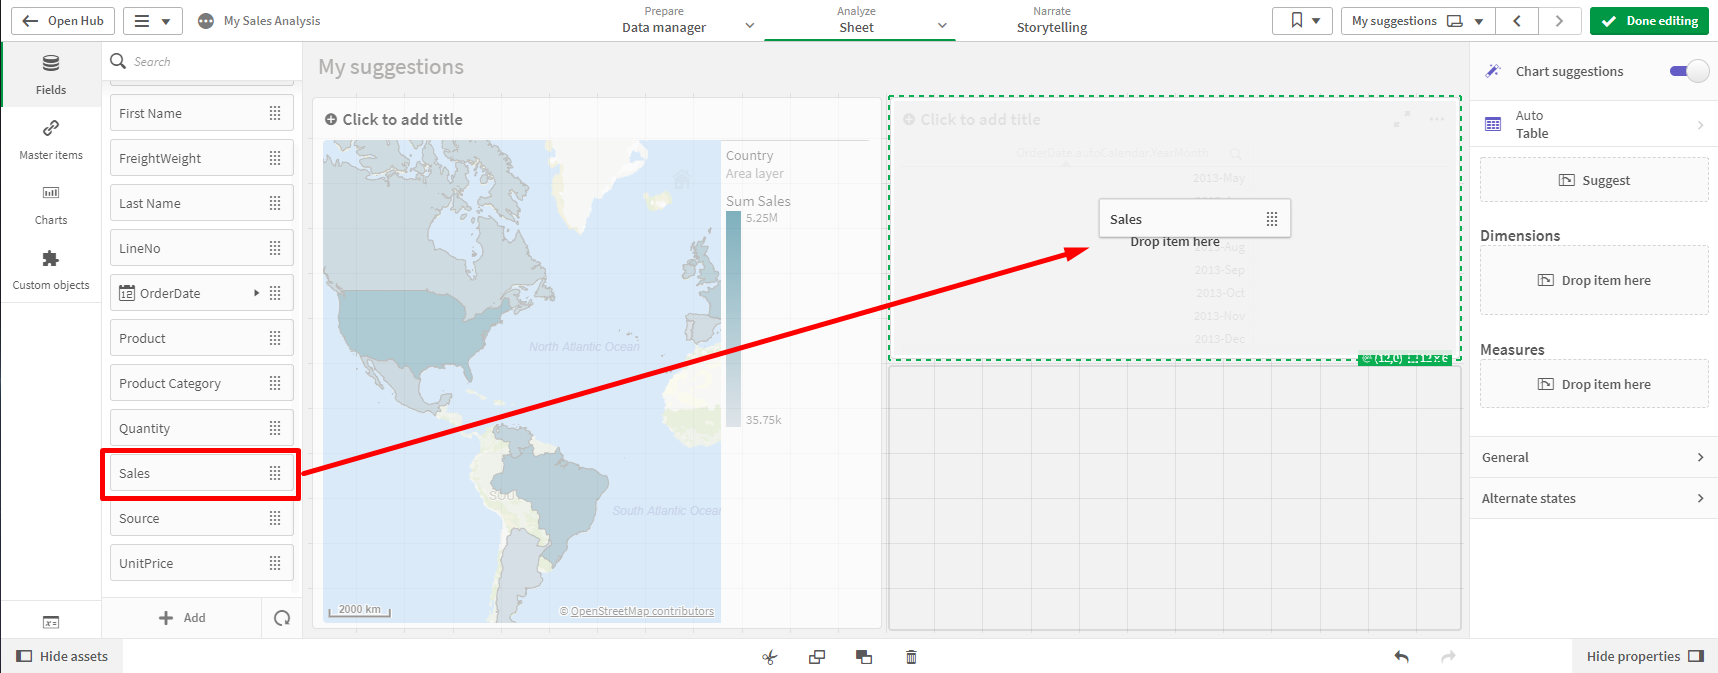
\includegraphics[width=13cm]{./img/img20.png}
        \end{center}
        \begin{itemize}
            \item Se obtiene un gráfico de líneas, debido al hecho de que se ha proporcionado una dimensión de fecha y un campo de valores de medida a esta visualización.
            \begin{center}
                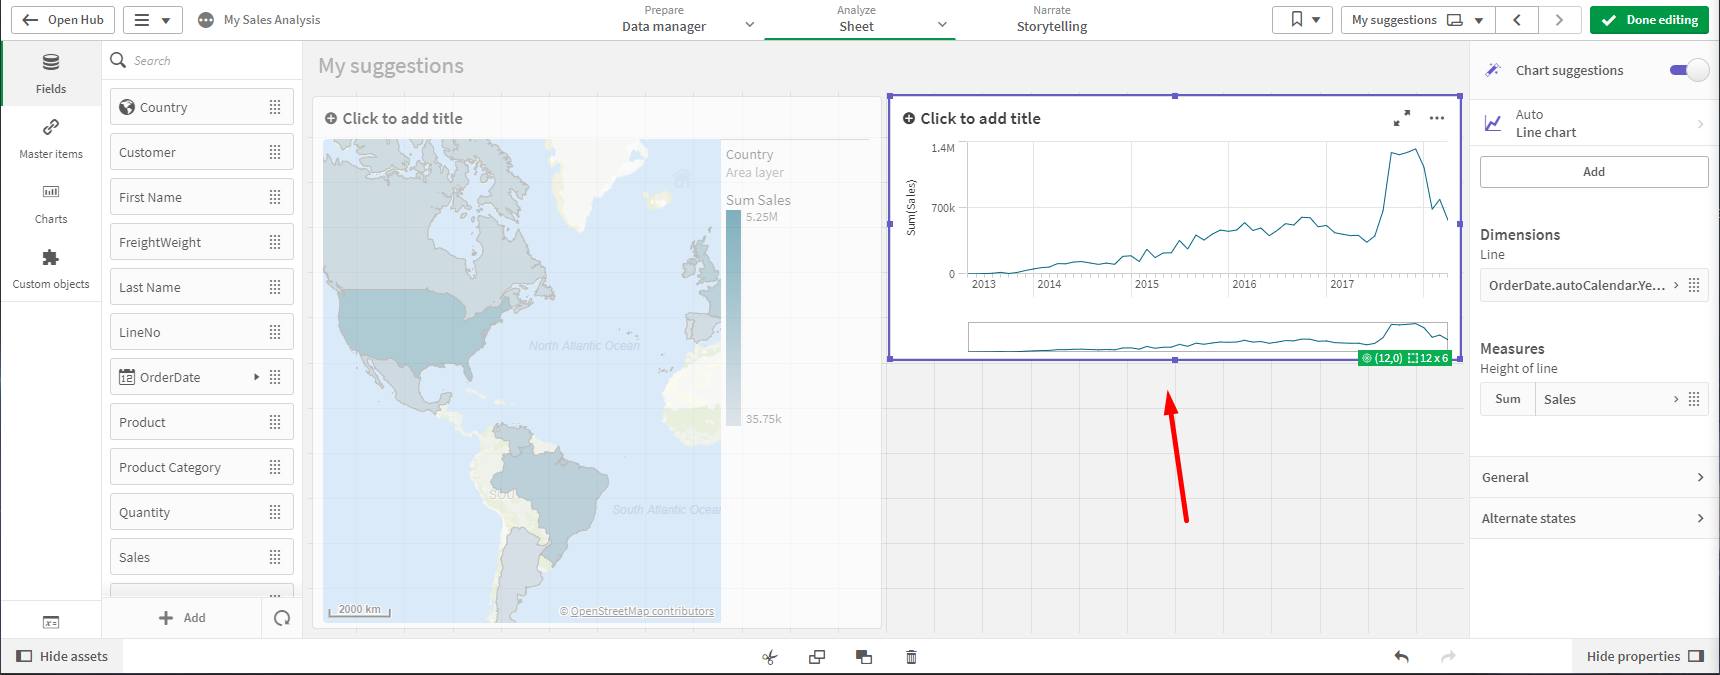
\includegraphics[width=13cm]{./img/img21.png}
            \end{center}
        \end{itemize}
        \item Arrastre y suelte el campo \textit{Quantity} para cubrir todo el gráfico de líneas.
        \begin{center}
            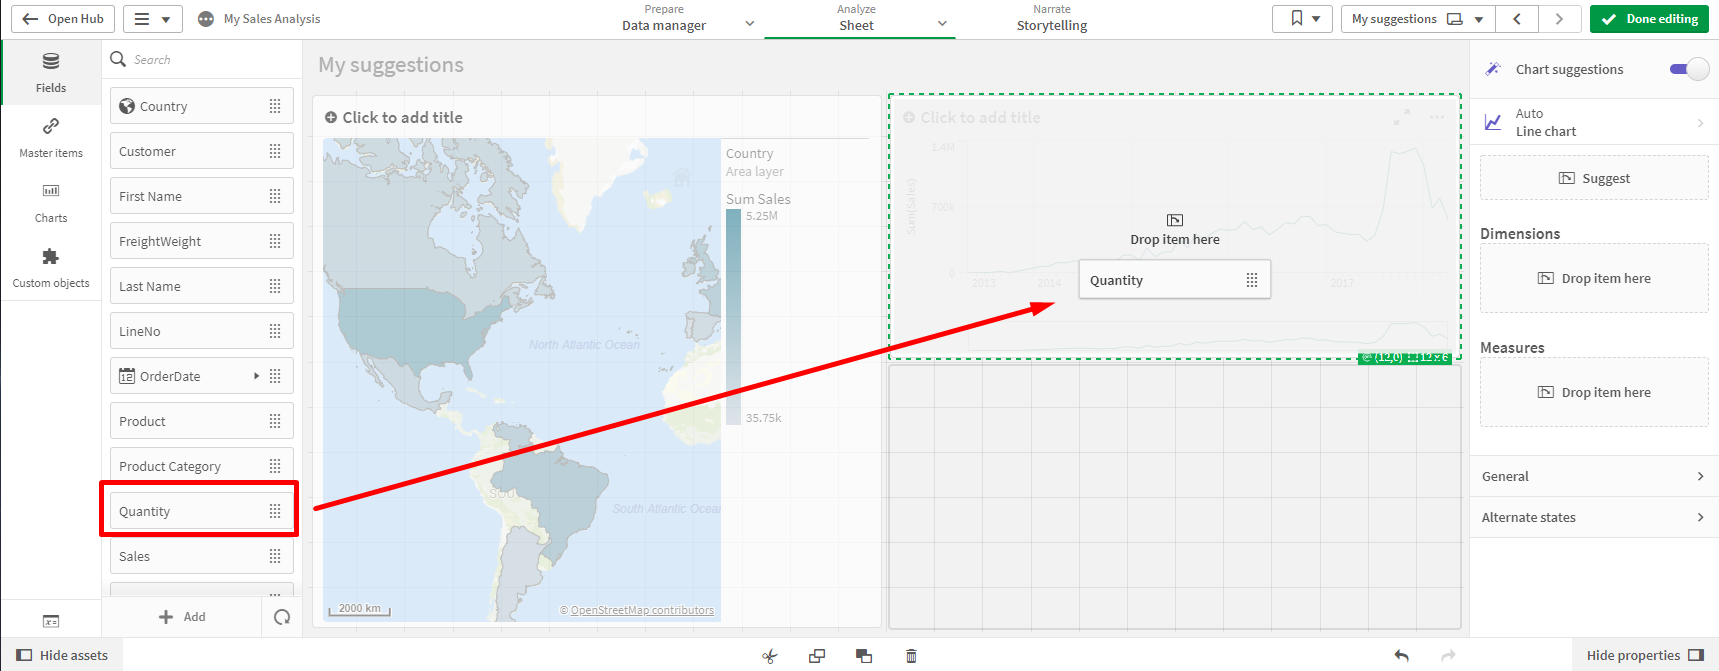
\includegraphics[width=13cm]{./img/img22.png}
        \end{center}
        \begin{itemize}
            \item 
            Se obtiene un gráfico combinado, debido al hecho de que se proporcionaron una dimensión y múltiples medidas (que ocupan diferentes rangos).
            \begin{center}
                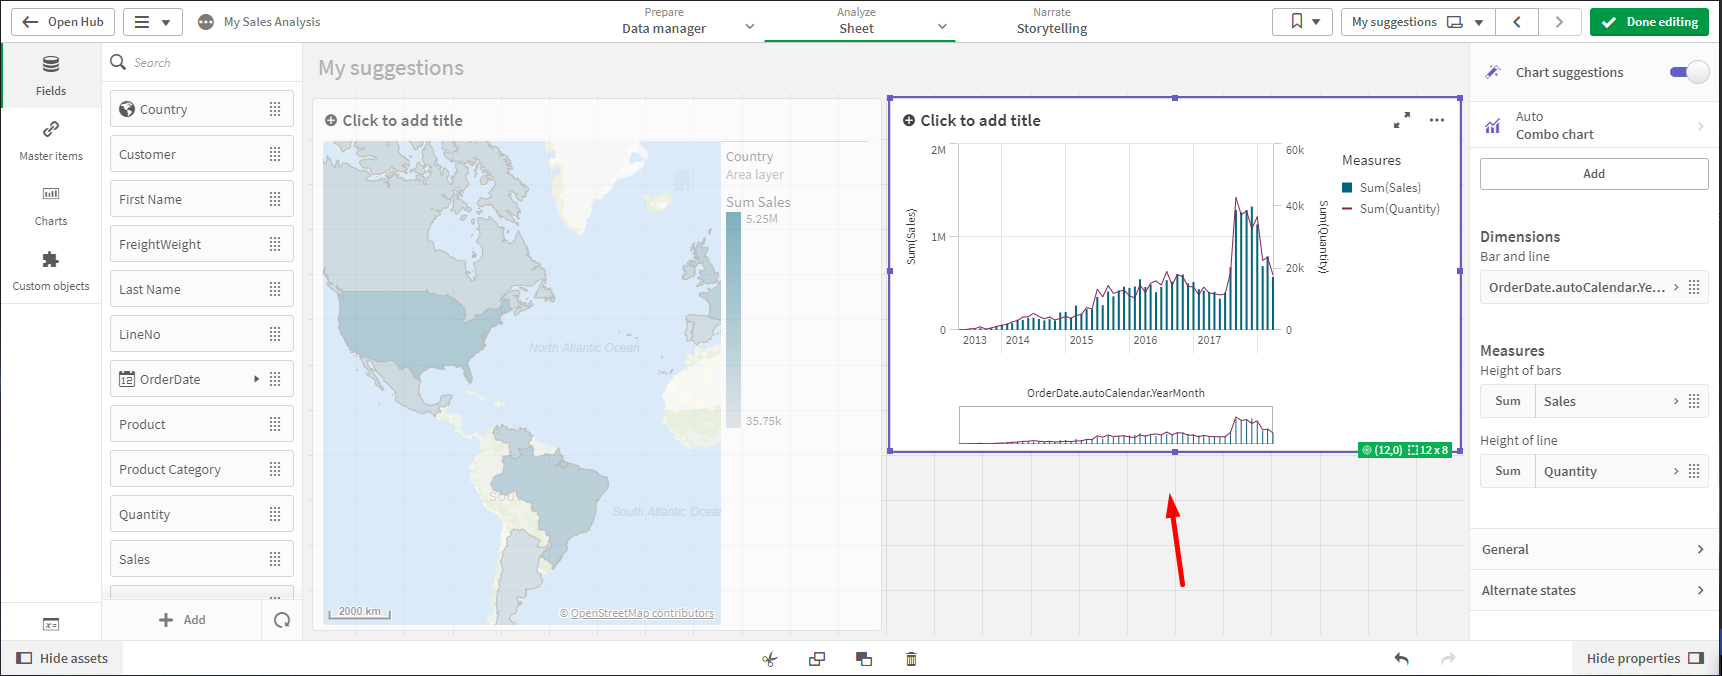
\includegraphics[width=13cm]{./img/img22.1.png}
            \end{center}
            \item Haga clic en el botón \textbf{Done editing}.
            \begin{center}
                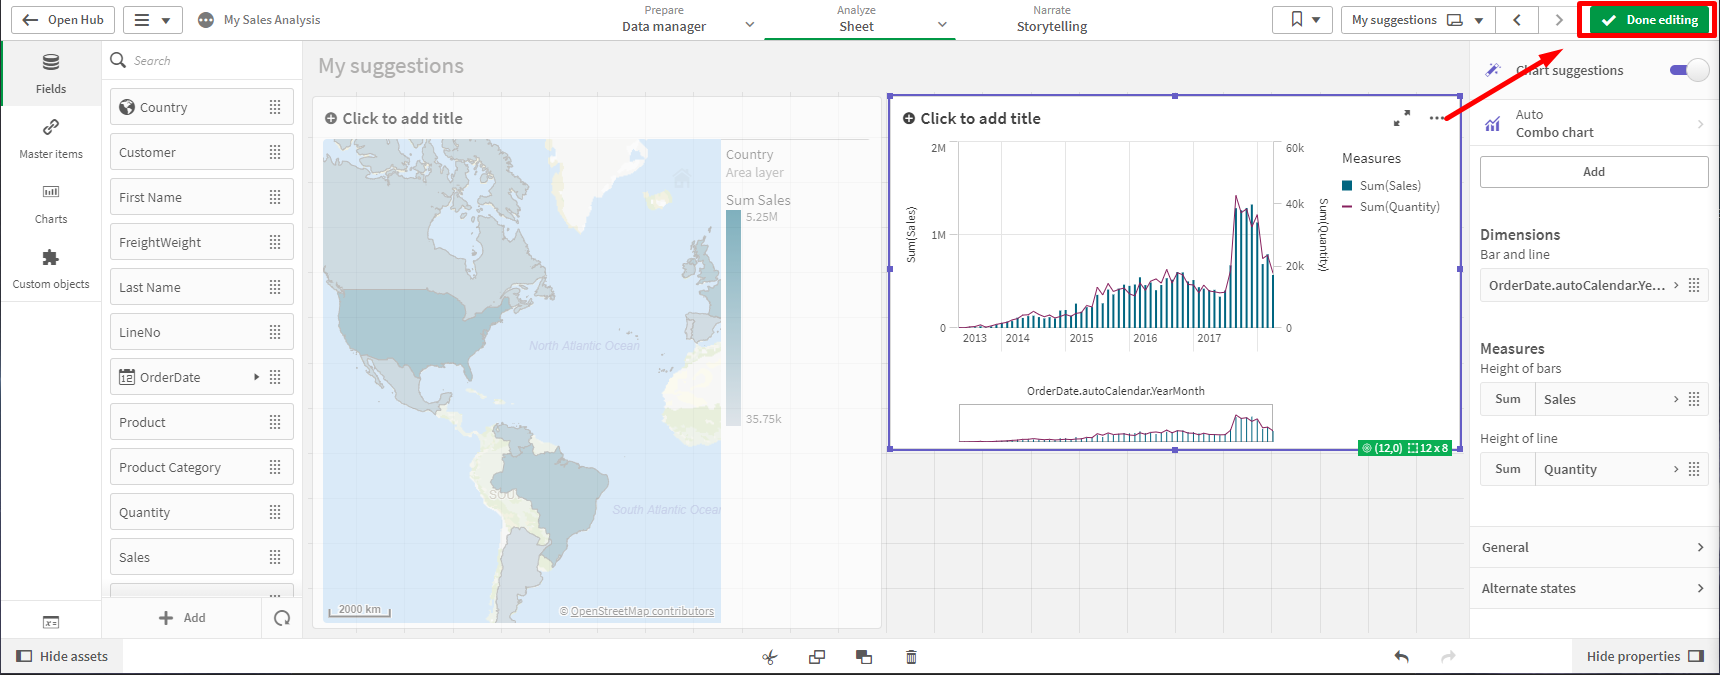
\includegraphics[width=13cm]{./img/img22.2.png}
            \end{center}
            \item Use el control deslizante de zoom del minigráfico, debajo del gráfico combinado, para examinar los valores más recientes de mes y año.
            \begin{center}
                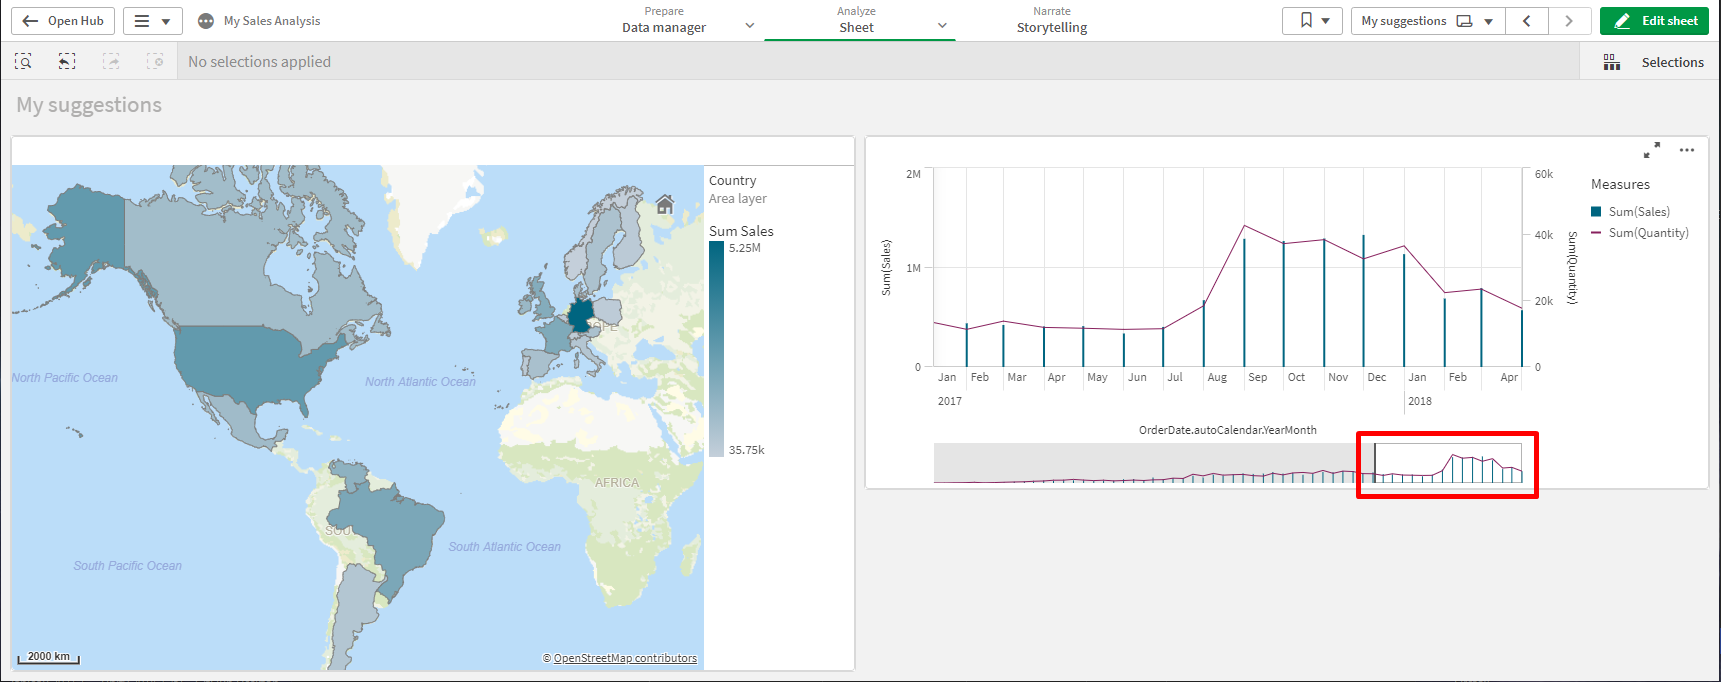
\includegraphics[width=13cm]{./img/img22.3.png}
            \end{center}
        \end{itemize}
    \end{enumerate}
    %%%%%%%%%%%%%%%%%%%%%%%%%%%%%%%%%%%%%%%%%%%%%%%%%%%%%%%%%%%%%%%%%%%%%%%%%%%%%%%%%%%%%%%%%%%%%%%%%%%%%%%%%%%%%%%%%%%%%%%%%%%%%%%%%%%%%%%%%%%%%%%%%%%%%%%%%%%%%%%%%%%%%%%%%%%%%%%%%%%%%%%%%%%%%%%%%%%%%%%%%%%%%%%%%%%%%%%%%%%%%%%%%%%%%%%%%%%%%%%%%%%%%%%%%%%%%%%%%%%%%%%%%%%%%%%%%%%%%%%%%%%%%%%%%%%%%%%%%%%%%%%%%%%%%%%%%%%%%%%%%%%%%%%%%%%%%%%%%%%%%%%%%%%%%%%%%%%%%%%%%%%%%%%%%%%%%%%%%%%%%%%%%%%%%%%%%%%%%%%%%%%%%%%%%%%%%%%%%%%%%%%%%%%%%%%%%%%%%%%%%%%%%%%%%%%%%%%%%%%%%%%%%%%%%%%%%%%%%%%%%%%%%%%%%%%%%%%
    \subsection{Pruebe un tipo de gráfico alternativo sugerido}
    \begin{enumerate}[\tab 1.]
        \item Vuelva al modo \textbf{Editar hoja} y considere sugerencias de gráficos alternativos.
        \begin{center}
            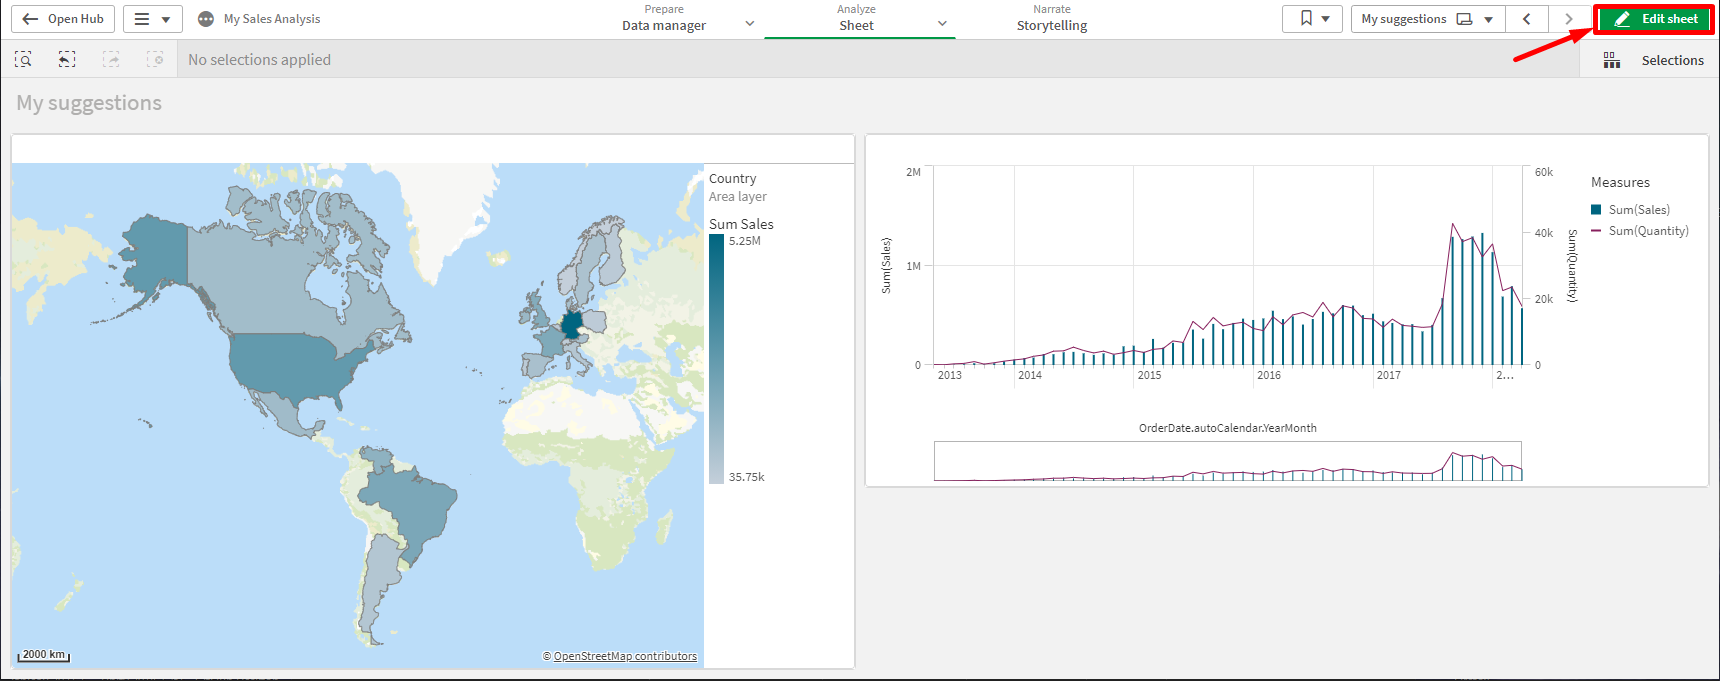
\includegraphics[width=13cm]{./img/img23.png}
        \end{center}
        \begin{itemize}
            \item Cambie del gráfico \textbf{Combo chart} a un \textbf{Line chart}.
            \begin{center}
                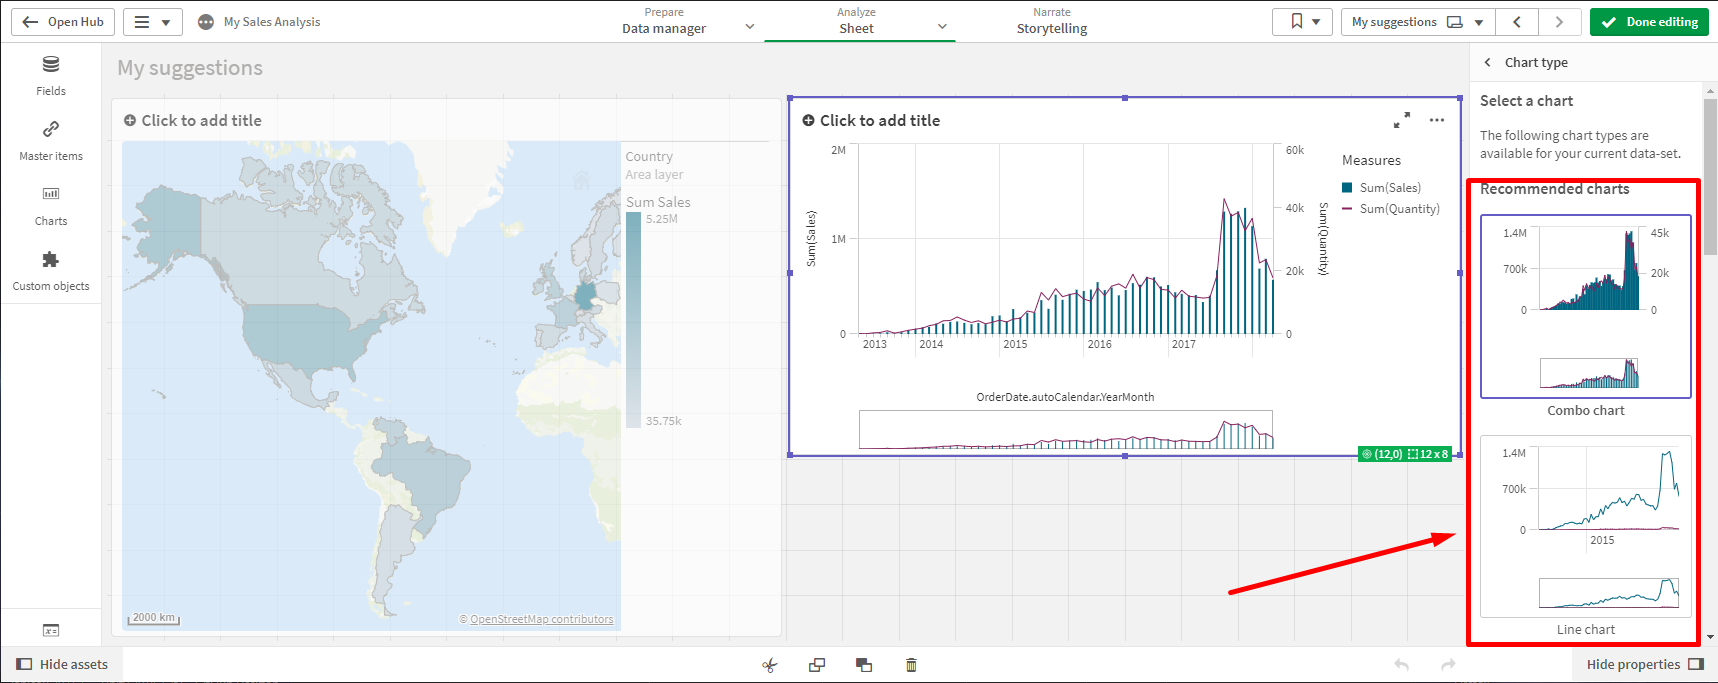
\includegraphics[width=13cm]{./img/img23.1.png}
            \end{center}
        \end{itemize}
    \end{enumerate}
    %%%%%%%%%%%%%%%%%%%%%%%%%%%%%%%%%%%%%%%%%%%%%%%%%%%%%%%%%%%%%%%%%%%%%%%%%%%%%%%%%%%%%%%%%%%%%%%%%%%%%%%%%%%%%%%%%%%%%%%%%%%%%%%%%%%%%%%%%%%%%%%%%%%%%%%%%%%%%%%%%%%%%%%%%%%%%%%%%%%%%%%%%%%%%%%%%%%%%%%%%%%%%%%%%%%%%%%%%%%%%%%%%%%%%%%%%%%%%%%%%%%%%%%%%%%%%%%%%%%%%%%%%%%%%%%%%%%%%%%%%%%%%%%%%%%%%%%%%%%%%%%%%%%%%%%%%%%%%%%%%%%%%%%%%%%%%%%%%%%%%%%%%%%%%%%%%%%%%%%%%%%%%%%%%%%%%%%%%%%%%%%%%%%%%%%%%%%%%%%%%%%%%%%%%%%%%%%%%%%%%%%%%%%%%%%%%%%%%%%%%%%%%%%%%%%%%%%%%%%%%%%%%%%%%%%%%%%%%%%%%%%%%%%%%%%%%%%
    \subsection{Cambie el interruptor de sugerencias de gráficos de ‘on’ a ‘off’}
    \begin{enumerate}[\tab 1.]
        \item Nos gustaría ajustar la combinación de colores aplicada a las formas de los países en el gráfico de mapa, así que cambie el interruptor de \textbf{Chart suggestions} a \textbf{‘off’}.
        \begin{center}
            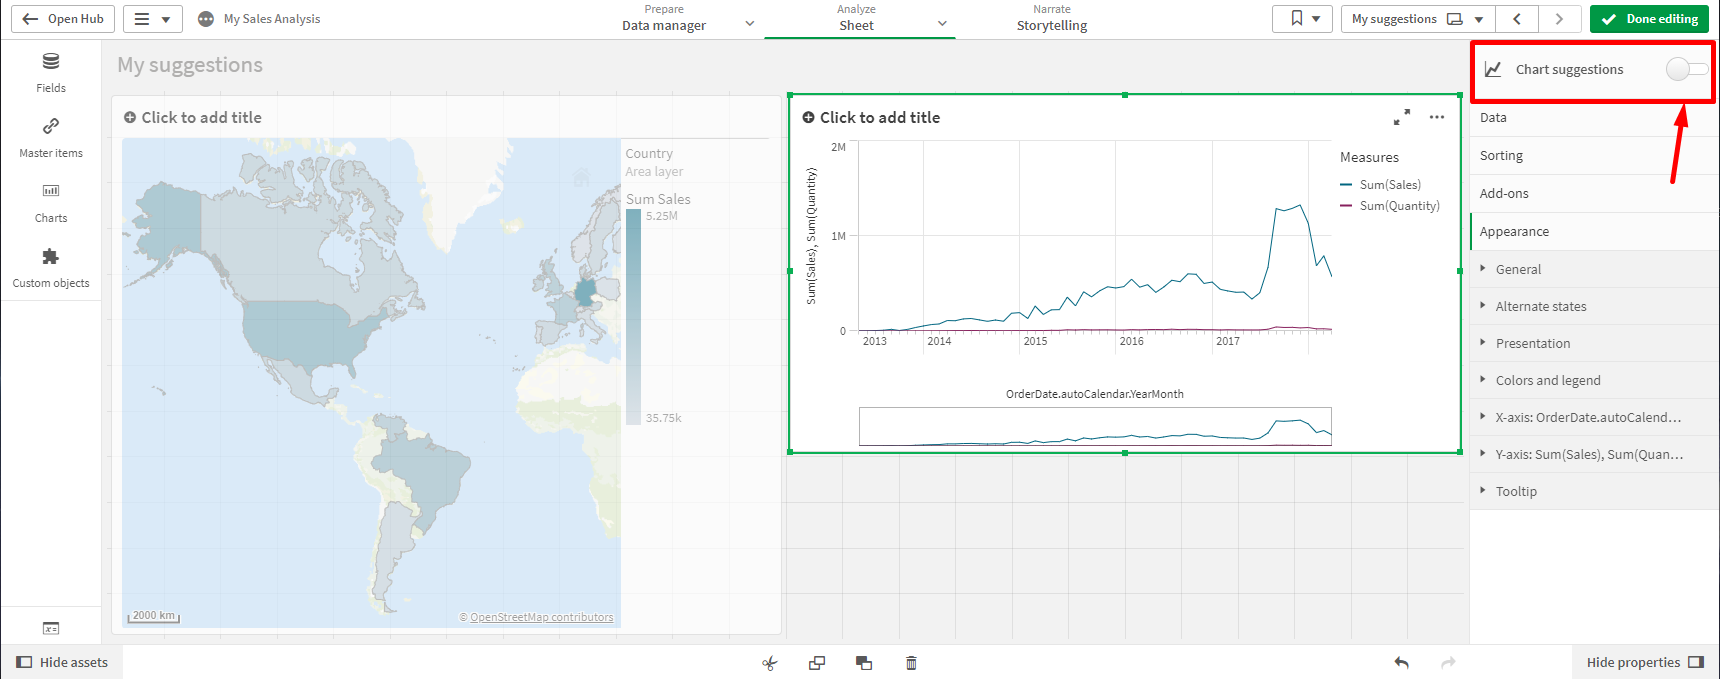
\includegraphics[width=13cm]{./img/img24.png}
        \end{center}
        \item Abra la sección \textbf{Layers} del panel de propiedades y haga clic en \textit{Area Layer} de \textbf{Country}.
        \begin{center}
            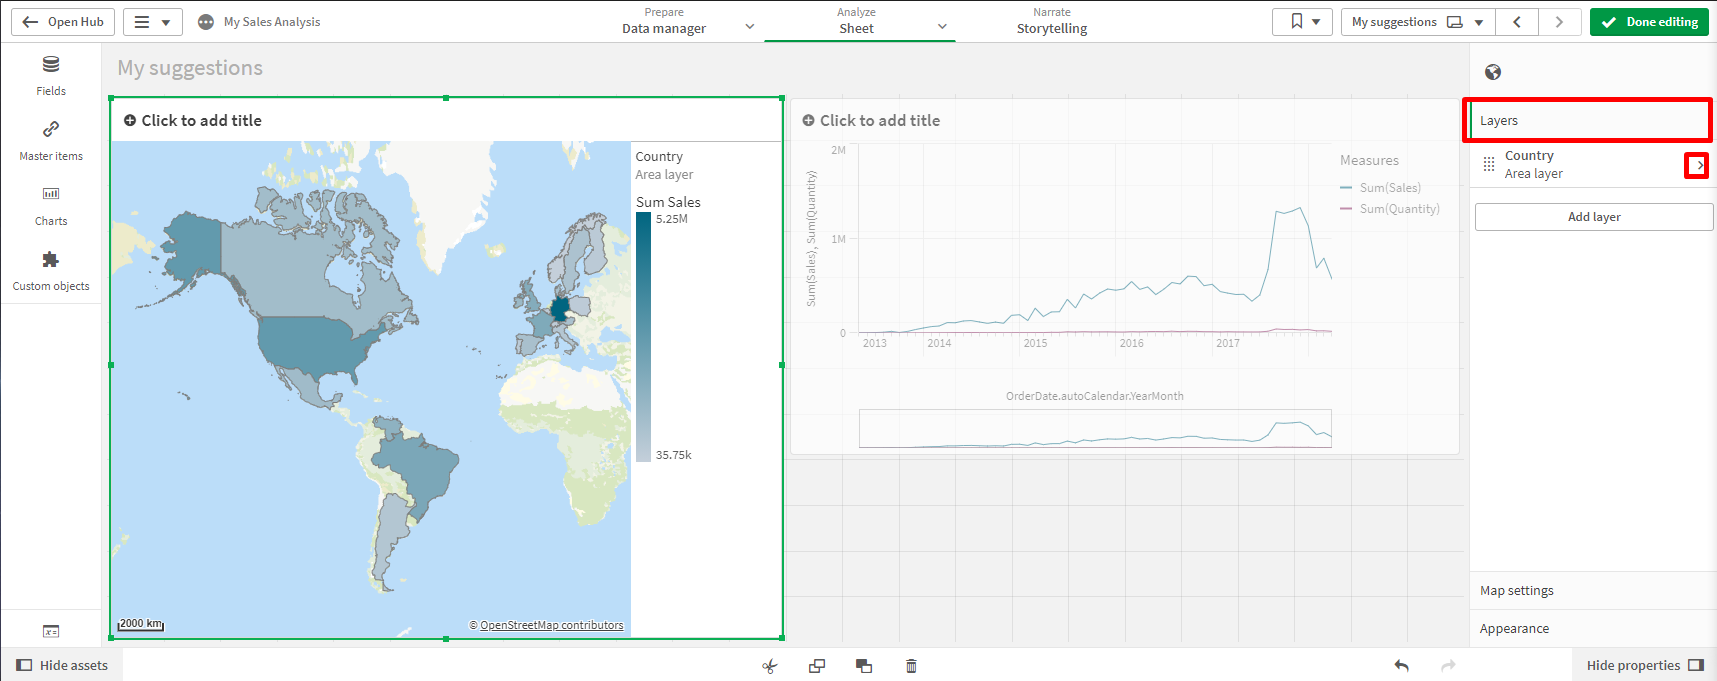
\includegraphics[width=13cm]{./img/img25.png}
        \end{center}
        \item Abra la sección \textbf{Colors} y busque la opcion \textbf{Color scheme}.
        \begin{center}
            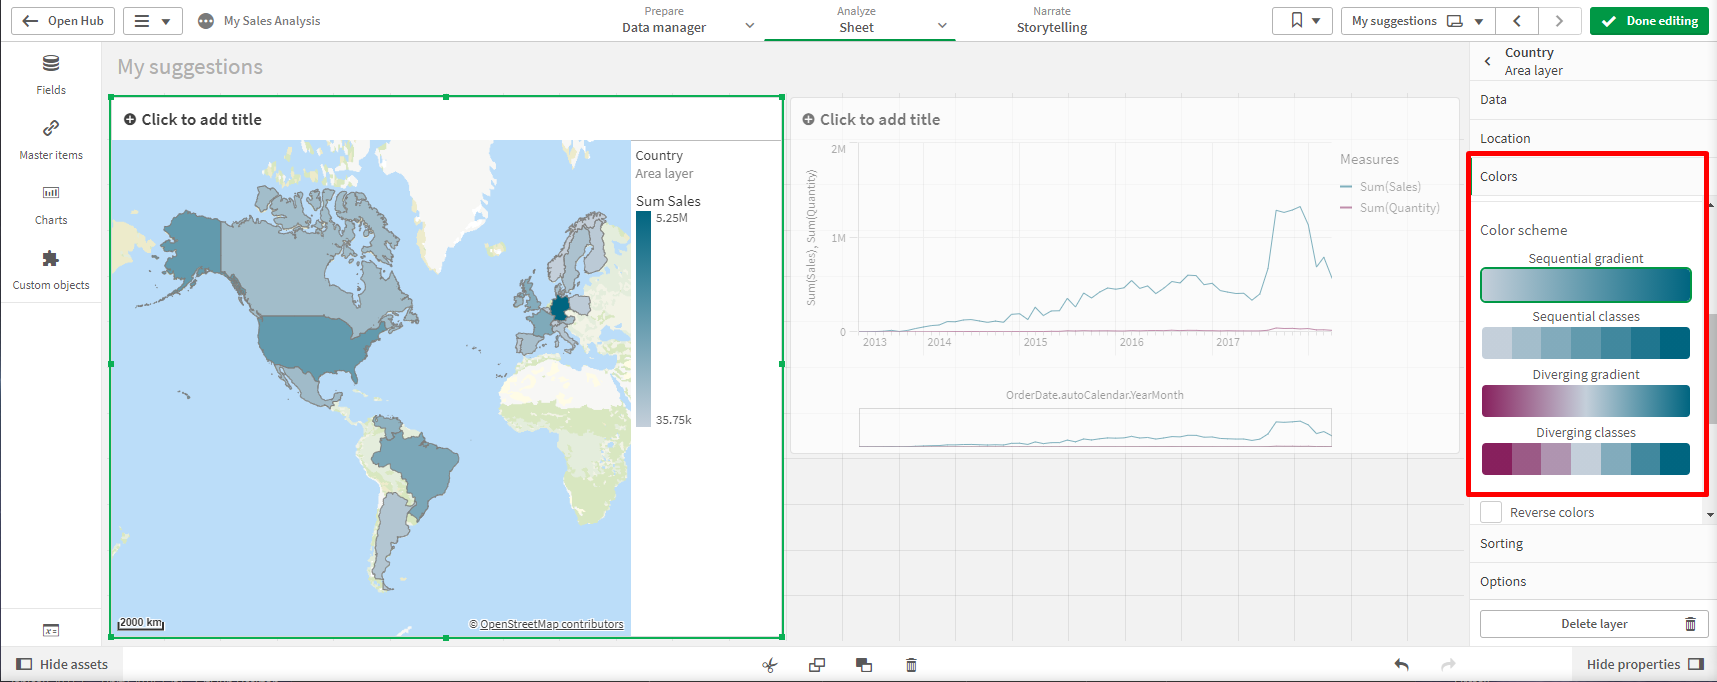
\includegraphics[width=13cm]{./img/img26.png}
        \end{center}
        \begin{itemize}
            \item Cambie el esquema de color de \textbf{Sequential gradient} a \textbf{Diverging gradient}.
            \begin{center}
                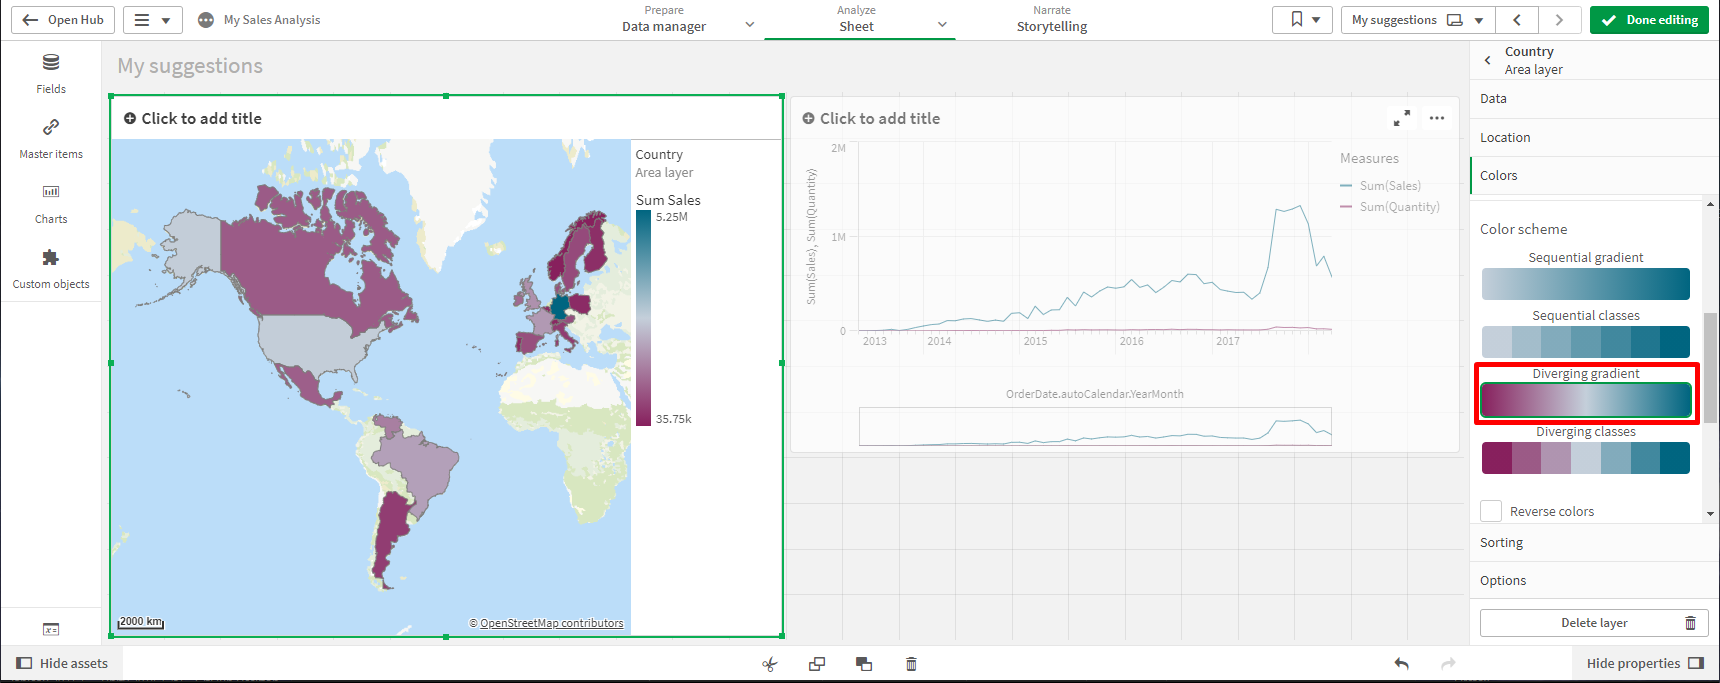
\includegraphics[width=13cm]{./img/img26.1.png}
            \end{center}
            \item Marque la casilla de verificación \textbf{Reverse colors}.
            \begin{center}
                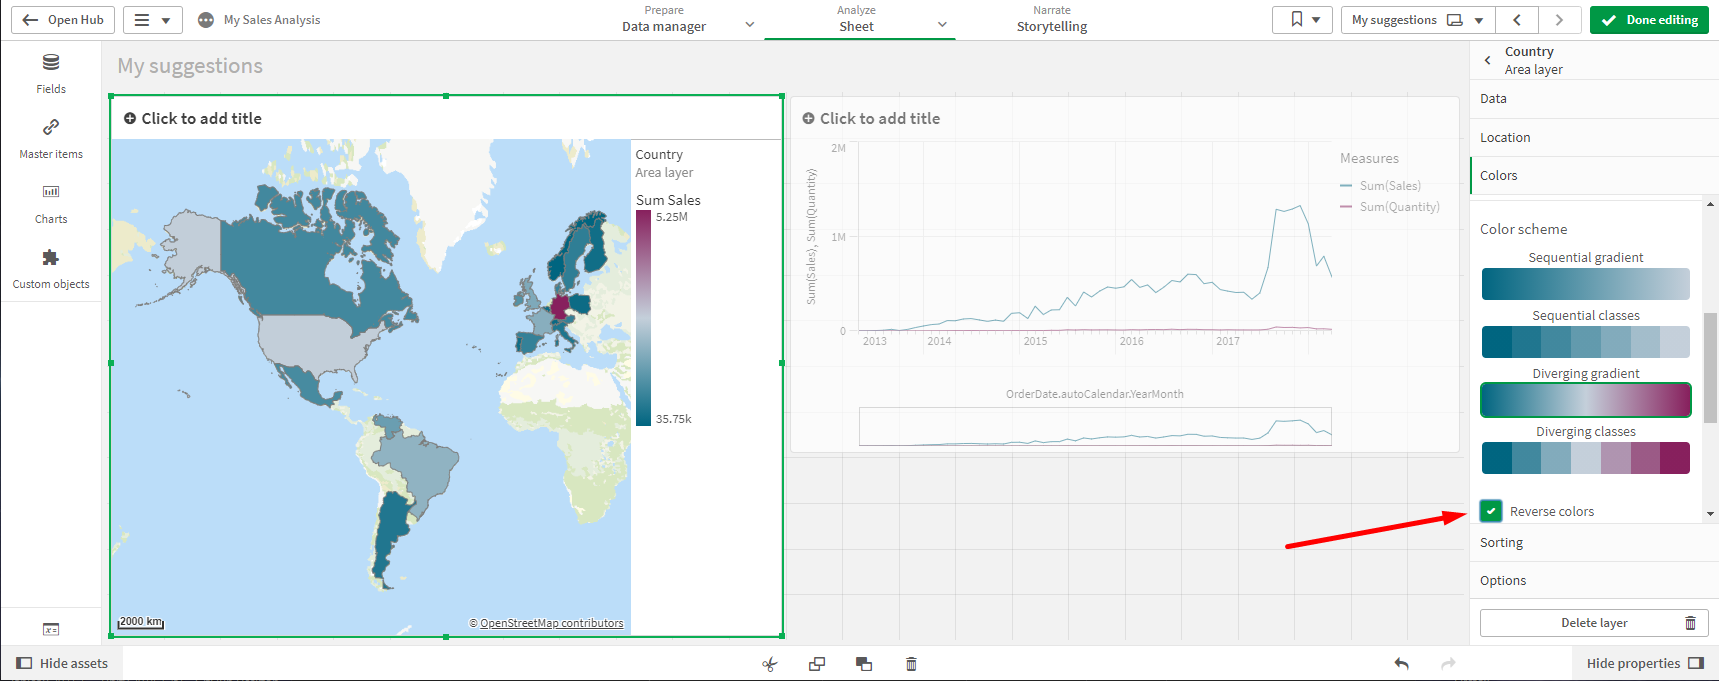
\includegraphics[width=13cm]{./img/img26.2.png}
            \end{center}
        \end{itemize}
        \item El mapa resultante debería aparecer como se ve a continuación..
        \begin{center}
            \includegraphics[width=13cm]{./img/img27.png}
        \end{center}
    \end{enumerate}
    %%%%%%%%%%%%%%%%%%%%%%%%%%%%%%%%%%%%%%%%%%%%%%%%%%%%%%%%%%%%%%%%%%%%%%%%%%%%%%%%%%%%%%%%%%%%%%%%%%%%%%%%%%%%%%%%%%%%%%%%%%%%%%%%%%%%%%%%%%%%%%%%%%%%%%%%%%%%%%%%%%%%%%%%%%%%%%%%%%%%%%%%%%%%%%%%%%%%%%%%%%%%%%%%%%%%%%%%%%%%%%%%%%%%%%%%%%%%%%%%%%%%%%%%%%%%%%%%%%%%%%%%%%%%%%%%%%%%%%%%%%%%%%%%%%%%%%%%%%%%%%%%%%%%%%%%%%%%%%%%%%%%%%%%%%%%%%%%%%%%%%%%%%%%%%%%%%%%%%%%%%%%%%%%%%%%%%%%%%%%%%%%%%%%%%%%%%%%%%%%%%%%%%%%%%%%%%%%%%%%%%%%%%%%%%%%%%%%%%%%%%%%%%%%%%%%%%%%%%%%%%%%%%%%%%%%%%%%%%%%%%%%%%%%%%%%%%%
    \subsection{Desarrollar una hoja sin ayuda}
    \begin{enumerate}[\tab 1.]
        \item Cree una nueva hoja en la aplicación, titulada \textbf{“My custom charts“}.
        \begin{center}
            \includegraphics[width=13cm]{./img/img28.png}
        \end{center}
        \item Arrastre y suelte objetos desde la sección Gráficos del panel de activos al área de visualización y cambie el tamaño de cada uno para completar una hoja con un \textbf{Bar chart}, \textbf{Table}, \textbf{Pie Chart}, \textbf{KPI}, \textbf{Filter pane} y \textbf{Text \& image} organizada dentro del espacio de visualización como se muestra a continuación:
        \begin{center}
            \includegraphics[width=13cm]{./img/img29.png}
        \end{center}
    \end{enumerate}
    %%%%%%%%%%%%%%%%%%%%%%%%%%%%%%%%%%%%%%%%%%%%%%%%%%%%%%%%%%%%%%%%%%%%%%%%%%%%%%%%%%%%%%%%%%%%%%%%%%%%%%%%%%%%%%%%%%%%%%%%%%%%%%%%%%%%%%%%%%%%%%%%%%%%%%%%%%%%%%%%%%%%%%%%%%%%%%%%%%%%%%%%%%%%%%%%%%%%%%%%%%%%%%%%%%%%%%%%%%%%%%%%%%%%%%%%%%%%%%%%%%%%%%%%%%%%%%%%%%%%%%%%%%%%%%%%%%%%%%%%%%%%%%%%%%%%%%%%%%%%%%%%%%%%%%%%%%%%%%%%%%%%%%%%%%%%%%%%%%%%%%%%%%%%%%%%%%%%%%%%%%%%%%%%%%%%%%%%%%%%%%%%%%%%%%%%%%%%%%%%%%%%%%%%%%%%%%%%%%%%%%%%%%%%%%%%%%%%%%%%%%%%%%%%%%%%%%%%%%%%%%%%%%%%%%%%%%%%%%%%%%%%%%%%%%%%%%%
    \subsection{Desarrolle una hoja sin ayuda (cont’d)}
    \begin{enumerate}[\tab 1.]
        \item Configuración \textbf{Bar chart}.
        \begin{enumerate}
            \item \textbf{Dimension} = \textit{Product Category}.
            \begin{center}
                \includegraphics[width=13cm]{./img/img30.1.png}
            \end{center}
            \item \textbf{Measure} = \textit{Sales}, aggregated with a sum: \textit{\textbf{Sum(Sales)}}.
            \begin{center}
                \includegraphics[width=13cm]{./img/img30.2.png}
            \end{center}
            \item Agregue un título al gráfico que diga: \textit{\textbf{“Sales totals per product category“}}.
            \begin{center}
                \includegraphics[width=13cm]{./img/img30.3.png}
            \end{center}
        \end{enumerate}
        \item Configuración \textbf{Table}.
        \begin{enumerate}
            \item \textbf{Dimension} = \textit{Product}.
            \begin{center}
                \includegraphics[width=13cm]{./img/img31.1.png}
            \end{center}
            \item Desde la sección Campos del panel de activos, arrastre y suelte el campo \textbf{Sales} para cubrir toda la tabla.
            \begin{center}
                \includegraphics[width=13cm]{./img/img31.2.png}
            \end{center}
            \begin{itemize}
                \item Agregar como \textbf{Measure}, agregar con una \textbf{Suma}: \textit{\textbf{sum(Sales)}}
                \begin{center}
                    \includegraphics[width=13cm]{./img/img31.3.png}
                \end{center}
                \item Utilice la sección \textbf{Data} del panel de propiedades para expandir la subsección de medida \textit{Sum of Sales} y formatee la suma de valores de ventas de la siguiente manera:
                \begin{center}
                    \includegraphics[width=13cm]{./img/img31.4.png}
                \end{center}
                \begin{itemize}
                    \item Formato de número = \textbf{Numbre}
                    \begin{center}
                        \includegraphics[width=13cm]{./img/img31.4.1.png}
                    \end{center}
                    \item Formateo = \textbf{Simple}; \textbf{1.000}.
                    \begin{center}
                        \includegraphics[width=13cm]{./img/img31.4.2.png}
                    \end{center}
                \end{itemize}
            \end{itemize}
        \end{enumerate}
        \item Configuración \textbf{Pie chart}.
        \begin{enumerate}
            \item \textbf{Dimension} (Slice) = \textit{Source}
            \begin{center}
                \includegraphics[width=13cm]{./img/img32.1.png}
            \end{center}
            \item  \textbf{Measure} (Angle) = \textit{Sales}, agregadas con una \textbf{Sum}: \textit{\textbf{Sum(Sales)}}.
            \begin{center}
                \includegraphics[width=13cm]{./img/img32.2.png}
            \end{center}
            \item Agregue un título al gráfico que diga: \textbf{“Sales for new vs. existing accounts“}.
            \begin{center}
                \includegraphics[width=13cm]{./img/img32.3.png}
            \end{center}
        \end{enumerate}
        \item Configuración \textbf{KPI}.
        \begin{enumerate}
            \item \textbf{Measure} = Sales, agregadas con una \textbf{Sum}: \textit{\textbf{Sum(Sales)}}.
            \begin{center}
                \includegraphics[width=13cm]{./img/img33.png}
            \end{center}
        \end{enumerate}
        \item Configuración \textbf{Filter pane}.
        \begin{enumerate}
            \item \textbf{Dimension} = \textit{OrderDate.Year}.
            \begin{center}
                \includegraphics[width=13cm]{./img/img34.1.png}
            \end{center}
            \item .Expanda la subsección de dimensión resultante y edite el \textbf{título} a: \textit{\textbf{“Year”}}.
            \begin{center}
                \includegraphics[width=13cm]{./img/img34.2.png}
            \end{center}
        \end{enumerate}
        \item Configuración \textbf{Text \& image}.
        \begin{enumerate}
            \item Ingrese el texto: \textit{\textbf{“Select a year of interest to limit data”}}.
            \begin{center}
                \includegraphics[width=13cm]{./img/img35.png}
            \end{center}
        \end{enumerate}
        \item La hoja que configuró debería aparecer como se ve a continuación:
        \begin{center}
            \includegraphics[width=13cm]{./img/img36.png}
        \end{center}
    \end{enumerate}
    %%%%%%%%%%%%%%%%%%%%%%%%%%%%%%%%%%%%%%%%%%%%%%%%%%%%%%%%%%%%%%%%%%%%%%%%%%%%%%%%%%%%%%%%%%%%%%%%%%%%%%%%%%%%%%%%%%%%%%%%%%%%%%%%%%%%%%%%%%%%%%%%%%%%%%%%%%%%%%%%%%%%%%%%%%%%%%%%%%%%%%%%%%%%%%%%%%%%%%%%%%%%%%%%%%%%%%%%%%%%%%%%%%%%%%%%%%%%%%%%%%%%%%%%%%%%%%%%%%%%%%%%%%%%%%%%%%%%%%%%%%%%%%%%%%%%%%%%%%%%%%%%%%%%%%%%%%%%%%%%%%%%%%%%%%%%%%%%%%%%%%%%%%%%%%%%%%%%%%%%%%%%%%%%%%%%%%%%%%%%%%%%%%%%%%%%%%%%%%%%%%%%%%%%%%%%%%%%%%%%%%%%%%%%%%%%%%%%%%%%%%%%%%%%%%%%%%%%%%%%%%%%%%%%%%%%%%%%%%%%%%%%%%%%%%%%%%%
    \subsection{Analizar una hoja}
    \begin{enumerate}[\tab 1.]
        \item Seleccione el año 2013, tome una instantánea del gráfico circular, anote con "2013".
        \begin{center}
            \includegraphics[width=13cm]{./img/img37.png}
        \end{center}
        \item Seleccione el año 2015 y tome una instantánea del gráfico circular, anote con "2015".
        \begin{center}
            \includegraphics[width=13cm]{./img/img38.png}
        \end{center}
        \item Haga clic para realizar las siguientes tres selecciones ...
        \begin{itemize}
            \item Seleccione la barra \textit{'Swimwear'} en el gráfico de barras y confirme la selección.
            \begin{center}
                \includegraphics[width=13cm]{./img/img39.1.png}
            \end{center}
            \item Seleccione el \textit{'año 2017'} en el panel de filtros y confirme la selección.
            \begin{center}
                \includegraphics[width=13cm]{./img/img39.2.png}
            \end{center}
            \item Seleccione la sección \textit{'New accounts'} en el gráfico circular y confirme la selección.
            \begin{center}
                \includegraphics[width=13cm]{./img/img39.3.png}
            \end{center}
        \end{itemize}
        \item Luego crear un bookmark con el nombre: \textit{\textbf{“New accounts, swimwear, 2017”}}.
        \begin{center}
            \includegraphics[width=13cm]{./img/img40.png}
        \end{center}
        \item Borre todas las selecciones y cree un segundo bookmark que limite las visualizaciones a los datos de 2014.
        \begin{center}
            \includegraphics[width=13cm]{./img/img41.png}
        \end{center}
        \item Nombrar el bookmark con el nombre: \textit{\textbf{“2014 orders”}}.
        \begin{center}
            \includegraphics[width=13cm]{./img/img42.png}
        \end{center}
    \end{enumerate}
    %%%%%%%%%%%%%%%%%%%%%%%%%%%%%%%%%%%%%%%%%%%%%%%%%%%%%%%%%%%%%%%%%%%%%%%%%%%%%%%%%%%%%%%%%%%%%%%%%%%%%%%%%%%%%%%%%%%%%%%%%%%%%%%%%%%%%%%%%%%%%%%%%%%%%%%%%%%%%%%%%%%%%%%%%%%%%%%%%%%%%%%%%%%%%%%%%%%%%%%%%%%%%%%%%%%%%%%%%%%%%%%%%%%%%%%%%%%%%%%%%%%%%%%%%%%%%%%%%%%%%%%%%%%%%%%%%%%%%%%%%%%%%%%%%%%%%%%%%%%%%%%%%%%%%%%%%%%%%%%%%%%%%%%%%%%%%%%%%%%%%%%%%%%%%%%%%%%%%%%%%%%%%%%%%%%%%%%%%%%%%%%%%%%%%%%%%%%%%%%%%%%%%%%%%%%%%%%%%%%%%%%%%%%%%%%%%%%%%%%%%%%%%%%%%%%%%%%%%%%%%%%%%%%%%%%%%%%%%%%%%%%%%%%%%%%%%%%
    \subsection{Contar una historia}
    \begin{enumerate}[\tab 1.]
        \item Utilice el menú de acceso rápido para navegar a la vista \textbf{Storytelling}.
        \begin{center}
            \includegraphics[width=13cm]{./img/img43.png}
        \end{center}
        \item Utilice la \textbf{Snapshot library} (icono de camara) para agregar las dos instantáneas que tomó a la diapositiva en blanco.
        \begin{center}
            \includegraphics[width=13cm]{./img/img44.png}
        \end{center}
        \item Utilice la \textbf{Text library} (icono A) para agregar una etiqueta para 2013 (al gráfico circular con la porción más pequeña de Cuentas nuevas)..
        \begin{center}
            \includegraphics[width=13cm]{./img/img45.png}
        \end{center}
        \item Agregue otra etiqueta para 2015 (al gráfico circular con el segmento de Cuentas Nuevas más grande).
        \begin{center}
            \includegraphics[width=13cm]{./img/img46.png}
        \end{center}
        \item Utilice la biblioteca de hojas para agregar la hoja titulada \textit{My suggestions} a una diapositiva de la historia.
        \begin{center}
            \includegraphics[width=13cm]{./img/img47.png}
        \end{center}
        \item Reproduce la historia.
        \begin{center}
            \includegraphics[width=13cm]{./img/img48.png}
        \end{center}
        \item Haga clic en diferentes aspectos visuales de su hoja de datos en vivo (como formas de países individuales) para ver que es una diapositiva interactiva.
        \begin{center}
            \includegraphics[width=13cm]{./img/img49.1.png}
        \end{center}
        \begin{center}
            \includegraphics[width=13cm]{./img/img49.2.png}
        \end{center}
    \end{enumerate}
    %%%%%%%%%%%%%%%%%%%%%%%%%%%%%%%%%%%%%%%%%%%%%%%%%%%%%%%%%%%%%%%%%%%%%%%%%%%%%%%%%%%%%%%%%%%%%%%%%%%%%%%%%%%%%%%%%%%%%%%%%%%%%%%%%%%%%%%%%%%%%%%%%%%%%%%%%%%%%%%%%%%%%%%%%%%%%%%%%%%%%%%%%%%%%%%%%%%%%%%%%%%%%%%%%%%%%%%%%%%%%%%%%%%%%%%%%%%%%%%%%%%%%%%%%%%%%%%%%%%%%%%%%%%%%%%%%%%%%%%%%%%%%%%%%%%%%%%%%%%%%%%%%%%%%%%%%%%%%%%%%%%%%%%%%%%%%%%%%%%%%%%%%%%%%%%%%%%%%%%%%%%%%%%%%%%%%%%%%%%%%%%%%%%%%%%%%%%%%%%%%%%%%%%%%%%%%%%%%%%%%%%%%%%%%%%%%%%%%%%%%%%%%%%%%%%%%%%%%%%%%%%%%%%%%%%%%%%%%%%%%%%%%%%%%%%%%%%
    \newpage
    \section{CONCLUSIONES}
    \begin{itemize}
        \item Se logro crear satisfactoriramente la aplicacion usando los componentes basicos que nos provee Qlik Sense, elaborando hojas con un asistente con un asistente y/o de manera nanual, hasta tener todos los datos organizados de la manera que se desea en un slide para una presenteacion.
        \item Qlik Sense es una herramienta poderosa de BI, que tiene una intuitiva interfaz para poder encontrar en los datos aquello que se nos escapa en un análisis convencional mediante consultas a una BD, y animándonos a siempre hacer preguntas adicionales al modelo mediante la selección, y a presentar los datos de diferentes maneras explotando la capacidad y flexibilidad del motor asociativo.
    \end{itemize}
    %%%%%%%%%%%%%%%%%%%%%%%%%%%%%%%%%%%%%%%%%%%%%%%%%%%%%%%%%%%%%%%%%%%%%%%%%%%%%%%%%%%%%%%%%%%%%%%%%%%%%%%%%%%%%%%%%%%%%%%%%%%%%%%%%%%%%%%%%%%%%%%%%%%%%%%%%%%%%%%%%%%%%%%%%%%%%%%%%%%%%%%%%%%%%%%%%%%%%%%%%%%%%%%%%%%%%%%%%%%%%%%%%%%%%%%%%%%%%%%%%%%%%%%%%%%%%%%%%%%%%%%%%%%%%%%%%%%%%%%%%%%%%%%%%%%%%%%%%%%%%%%%%%%%%%%%%%%%%%%%%%%%%%%%%%%%%%%%%%%%%%%%%%%%%%%%%%%%%%%%%%%%%%%%%%%%%%%%%%%%%%%%%%%%%%%%%%%%%%%%%%%%%%%%%%%%%%%%%%%%%%%%%%%%%%%%%%%%%%%%%%%%%%%%%%%%%%%%%%%%%%%%%%%%%%%%%%%%%%%%%%%%%%%%%%%%%%%
    \newpage
    \section{WEBGRAFIA}
    \begin{itemize}
        \item Qlik. (2020). Getting Started with Qlik Sense (QS Apr 2020).\\
        Recuperado de \textcolor{azul}{\url{https://learning.qlik.com/course/view.php?id=1527}}
        \item YouTube. (2019). Qlik Sense Basic Tutorial for beginners [Complete Tutorial] - Getting started - Part-1-of-10.\\
        Recuperado de \textcolor{azul}{\url{https://www.youtube.com/watch?v=zs24DVVIALU&list=PL6_D9USWkG1CvXmMXE24Ax38iyHvos7HO&index=1&ab_channel=AbhishekAgarrwal}}
        \item YouTube. (2019). Qlik Sense Basic Tutorial for beginners [Complete Tutorial] - Getting started - Part-2-of-10.\\
        Recuperado de \textcolor{azul}{\url{https://www.youtube.com/watch?v=Rz3qZguAkdA&list=RDCMUCxNzLV0gP8nuOZcSfyc0hsg&index=1&ab_channel=AbhishekAgarrwal}}
        \item YouTube. (2019). Qlik Sense Basic Tutorial for beginners [Complete Tutorial] - Getting started - Part-3-of-10.\\
        Recuperado de \textcolor{azul}{\url{https://www.youtube.com/watch?v=MbVwy3rPR7s&list=PL6_D9USWkG1CvXmMXE24Ax38iyHvos7HO&index=3&ab_channel=AbhishekAgarrwal}}
    \end{itemize}
\end{document}